\label{optimize_e051}

We've discussed how frontend generates symbol table and 3 address codes
from C program text until chapter \ref{stmt_e006}. In this chapter,
we'll discuss how frontend generates better symbol table and 3 address codes.

As we described at chapter \ref{stmt_e006},
when grammer symbol {\tt{function-definition}} is reduced
while bottom-up parsing, symbol table and 3 address codes are obtained
like bellow.

\begin{verbatim}
%{
/* yacc program text */
vector<tac*> code;
struct scope {
  ...
  static scope root;
};
%}

%%
...
function_definition
  : function_header compound_statement
    { function_definition($2); }
...
%%
void function_definition(comp_stmt* cs)
{
  cs->gen(); /* Genereate 3 address codes into global container `code' */
  ...
  if ( !error::counter )
    optimize(code);

  backend(&scope::root,code,...);  // Output symbol table and
                                   // 3 address codes to backend.
  ...
}
\end{verbatim}

\section{Unreferenced label}
\label{optimize_e003}
At \ref{_3ac_e002}, label are expressed class `{\tt{to3ac}}'
which contains referencing jump code in the member `{\tt{to3ac::m\_goto}}'.
So, we can easily know whether the label is referenced or not.
And if not, the label is erased like bellow.
\begin{verbatim}
void erase_to3ac(vector<tac*>& v)
{
  for ( p = v.begin() ; p != v.end() ; ) {
    to3ac* to = dynamic_cast<to3ac*>(*p);
    if ( !to ) {
      ++p;
      continue; 
    }
    if ( !to->m_goto.empty() ) {
      ++p;
      continue; 
    }
    p = v.erase(p);
  }
}
\end{verbatim}

\section{Basic block optimization}
\label{optimize_e058}
Chapter 9 of bibliography \cite{doragon} says about 
the way of basic block optimization. Basic block
is expressed like bellow.
\begin{verbatim}
struct basic_block {
  tac** m_leader;                  // Leader of this basic block
  int m_size;                      // Size of this basic block
  vector<basic_block*> m_preceed;  // Preceed basic blocks
  vector<basic_block*> m_follow;   // Following basic blocks
};
\end{verbatim}

\subsection{Division into basic blocks}

Bibliography \cite{doragon} algorithm 9.1 says about 
division into basic blocks. Now here, If the 3 address
code is one of {\tt{return}}, {\tt{call}},
and {\tt{*y := z}}, we additionally
make it  a leader of basic block.
For example,
\begin{verbatim}
int f(int* a, int* b, int n)
{
  int prod = 0;
  for ( int i = 0 ; i < n ; ++i )
    prod += a[i] * b[i];
  return prod;
}
\end{verbatim}
for above program, 3 address codes become like bellow.
\begin{verbatim}
f:
    prod := 0
    i := 0
  label0:
    if i >= n goto label1
    t0 := 4 * i
    t1 := a + t0
    t2 := 4 * i
    t3 := b + t2
    t4 := *t1
    t5 := *t3
    t6 := t4 * t5
    t7 := prod + t6
    prod := t7
    i := i + 1
    t8 := i
    goto label0
  label1:
    t9 := prod
    return t9
\end{verbatim}
These 3 address codes are devided into basic blocks illustrated
figure \ref{optimize_e000}.
\begin{figure}[htbp]
\begin{center}
%%\begin{htmlonly}
%%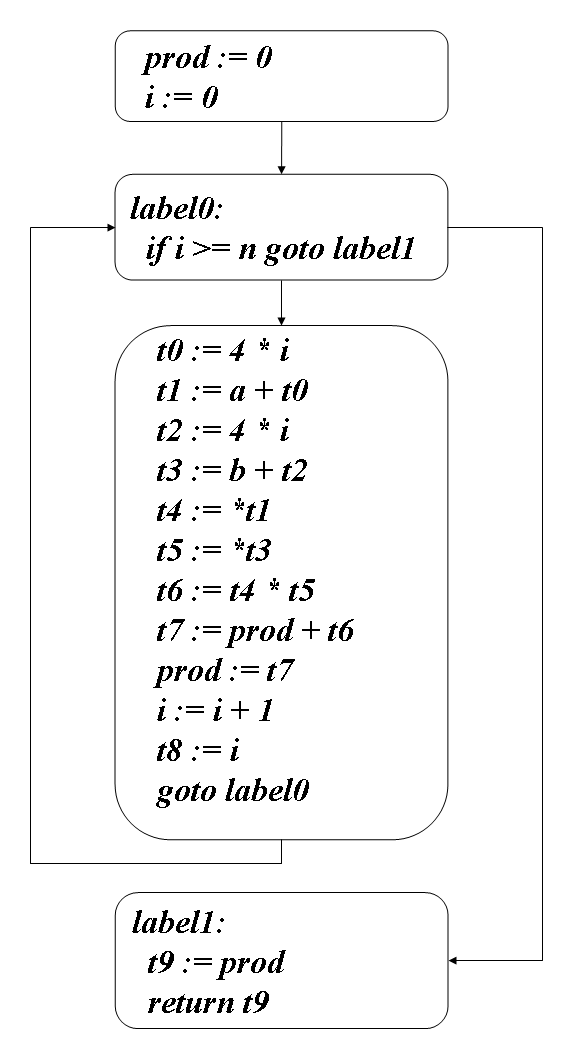
\includegraphics[width=0.8\linewidth,height=1.436\linewidth]{basic_block.png}
%%\end{htmlonly}
%%\begin{latexonly}
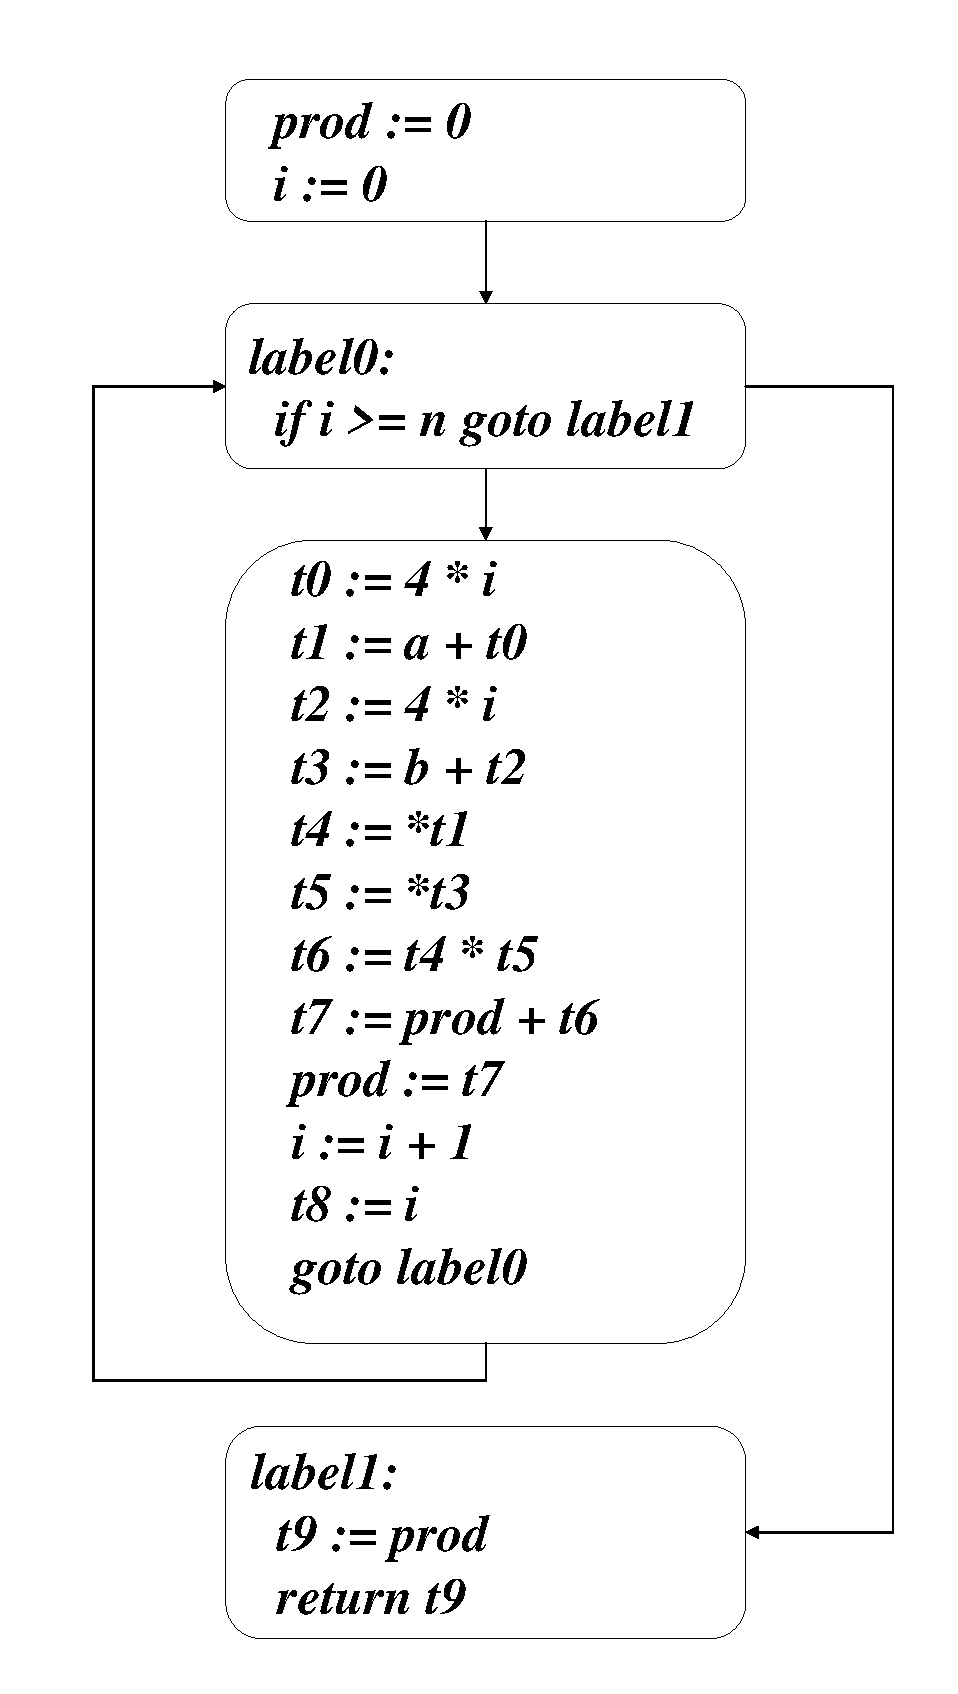
\includegraphics[width=0.8\linewidth,height=1.436\linewidth]{basic_block.eps}
%%\end{latexonly}
\caption{Division into basic blocks}
\label{optimize_e000}
\end{center}
\end{figure}

\subsection{Alive medium variable beyond basic block}

\label{optimize_e004}
Bibliography \cite{doragon} 9.5 says like bellow.
\begin{quote}
However if medium code generation algorithm or optimization algorithm
uses the same temporary variables through some basic blocks,
it is necessary to assume that they are alive beyond the basic blocks.
For this, mark such temporary variables specially, and distinguish
alive or death of temporary variables.
\end{quote}
Here, let's think about the medium variable which is alive beyond
basic block and is generated by the algorithm discussed in \ref{expr_e000}.
For example,
\begin{verbatim}
int f(int a, int b, int c){ return a * b + !c; }
\end{verbatim}
for this program, 3 address codes become like bellow.
\begin{verbatim}
f:
  t0 := a * b
  if c != 0 goto label1
  t1 := 1
  goto label2
label1:
  t1 := 0
label2
  t2 := t0 + t1
  return t2
\end{verbatim}
These 3 address codes are diveded into basic block illustrated in
figure \ref{optimize_e001}.
\begin{figure}[htbp]
\begin{center}
%%\begin{htmlonly}
%%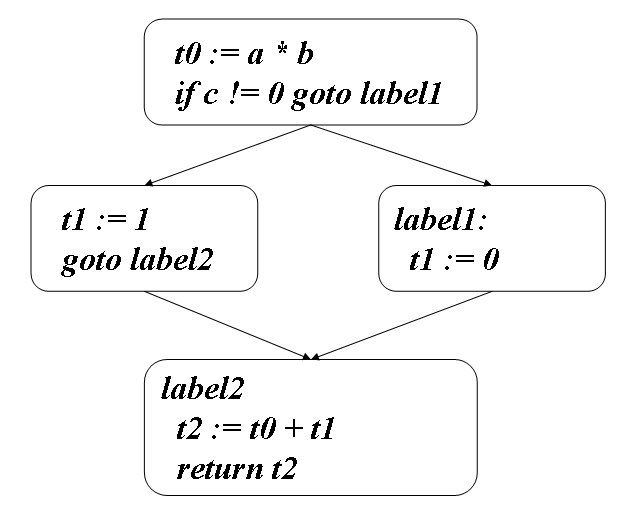
\includegraphics[width=0.89\linewidth,height=1.0\linewidth]{beyond_medium.png}
%%\end{htmlonly}
%%\begin{latexonly}
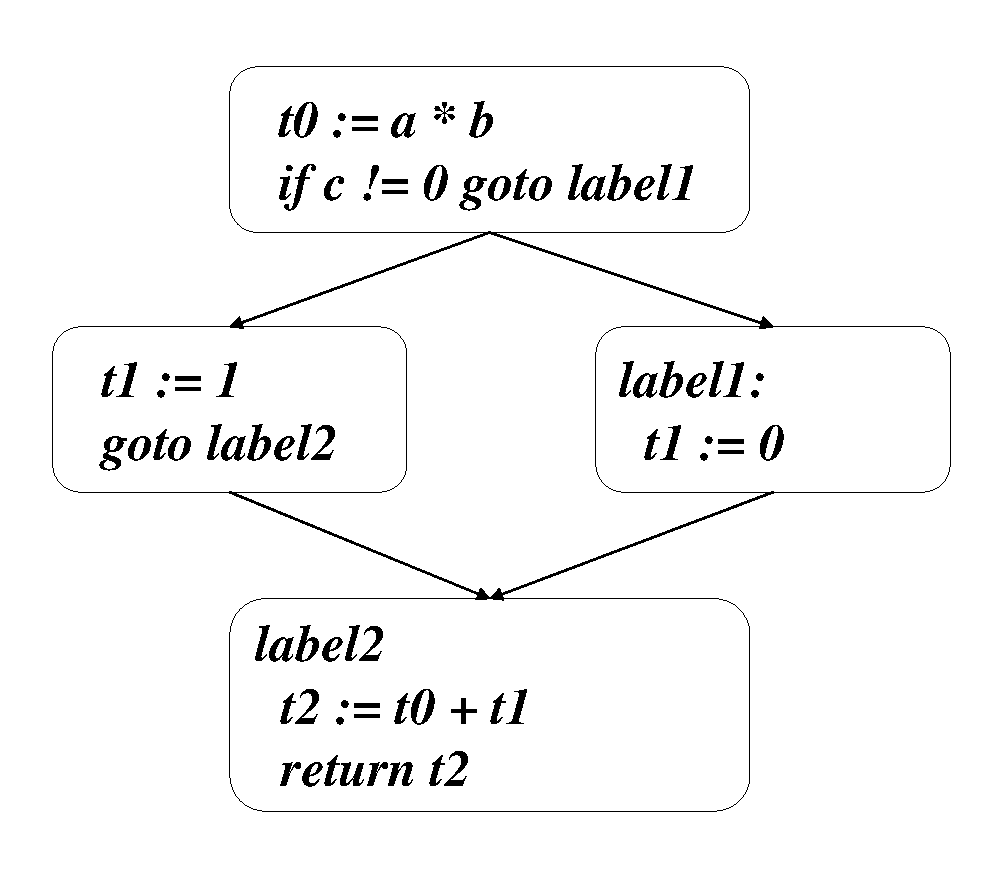
\includegraphics[width=0.89\linewidth,height=1.0\linewidth]{beyond_medium.eps}
%%\end{latexonly}
\caption{Alive medium variable beyond basic block}
\label{optimize_e001}
\end{center}
\end{figure}
`{\tt{t1}}' is alive beyond basic blocks. And please
note that `{\tt{t0}}' is also alive beyond basic blocks.
Generally, for binary operator $@$ and expression $expr_0 @ expr_1$,
if the result of $expr_1$ is alive beyond basic blocks,
then the result of $expr_0$ is also  alive beyond basic blocks.
\begin{verbatim}
void bin_expr::eval(expr* left, expr* right)
{
  var* y = left->eval();
  y = y->rvalue();
  var* z = right->eval();
  z = z->rvalue();
  if ( z->m_beyond ) {
    // Marked specially. i.e. `z' is alive beyond basic blocks.
    // Now mark `y' specially.
    y->m_beyond = true;
  }
  ...
  var* x = y->vf(z);
  ...
  return x;
  // `x' is not still marked specially. But if some operator is
  // applied to `x', it may be marked specially. i.e. We cannot
  // assume `x' is not alive beyond basic block.
}
\end{verbatim}
If frontend doesn't analize alive variables which are in program text
and frontend assumes that they are alive beyond basic blocks,
frontend has to assume that all medium variables may be alive beyond
basic block. That is, all medium variables are marked specially and
they are alive beyond basic blocks.

\subsection{Analisis alive variables}

Bibliography \cite{doragon} algorithm 10.4 says about 
analisis alive variables, and here, we'll take this way.
Consider bellow program please.
\begin{verbatim}

extern int a[];

void quicksort(int m, int n)
{
  if ( n <= m ) return;
  int i = m - 1;
  int j = n;
  int v = a[n];
  while ( 1 ) {
    do i = i + 1; while ( a[i] < v );
    do j = j - 1; while ( a[j] > v );
    if ( i >= j ) break;
    int x = a[i]; a[i] = a[j]; a[j] = x;
  }
  int y = a[i]; a[i] = a[n]; a[n] = y;
  quicksort(m,j); quicksort(i+1,n);
}
\end{verbatim}
For this program, generate symbol table and 3 addres codes
and then erase unreferenced label described in \ref{optimize_e003},
3 address codes become like bellow.
\begin{verbatim}
quicksort:                  label4:
  if n > m goto label0        t10 := 4 * i
  return                      t11 := a[t10]
label0:                       x := t11
  t0 := m - 1                 t12 := 4 * i
  i := t0                     t13 := 4 * j
  t1 := n                     t14 := a[t13]
  j := t1                     a[t12] := t14
  t2 := 4 * n                 t15 := 4 * j
  t3 := a[t2]                 t16 := x
  v := t3                     a[t15] := t16
label1:                       goto label1
label2:                     label5:
  t4 := i + 1                 t17 := 4 * i
  i := t4                     t18 := a[t17]
  t5 := 4 * i                 y := t18
  t6 := a[t5]                 t19 := 4 * i
  if t6 < v goto label2       t20 := 4 * n
label3:                       t21 := a[t20]
  t7 := j - 1                 a[t19] := t21
  j := t7                     t22 := 4 * n
  t8 := 4 * j                 t23 := y
  t9 := a[t8]                 a[t22] := t23
  if t9 > v goto label3       t24 := m
  if i < j goto label4        t25 := j
  goto label5                 param t24
                              param t25
                              call quicksort
                              t26 := i + 1
                              t27 := n
                              param t26
                              param t27
                              call quicksort
\end{verbatim}
These 3 address codes are dived into basic blocks illustrated in
figure \ref{optimize_e002}.
\begin{figure}[htbp]
\begin{center}
%%\begin{htmlonly}
%%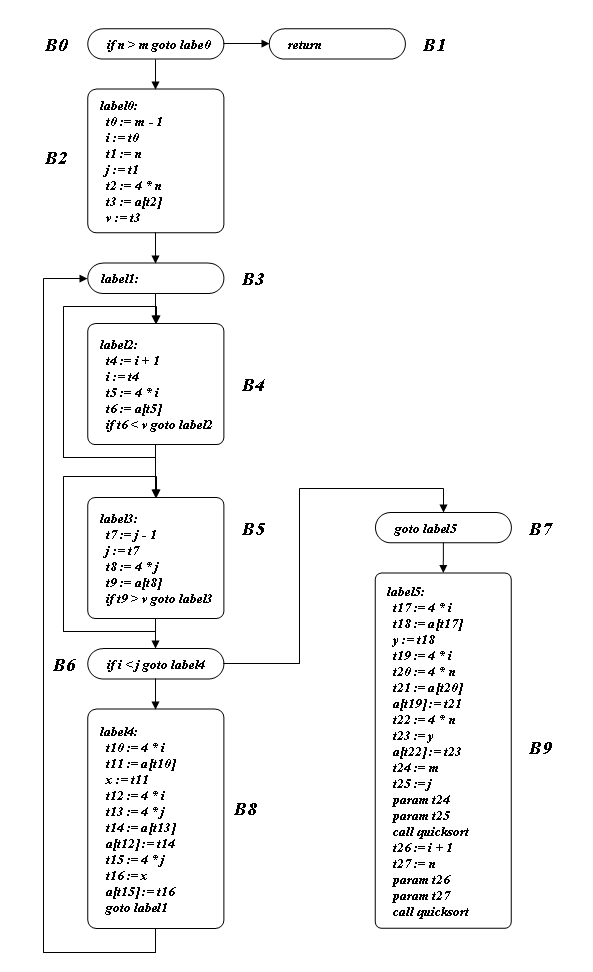
\includegraphics[width=1.01\linewidth,height=1.75\linewidth]{quicksort.png}
%%\end{htmlonly}
%%\begin{latexonly}
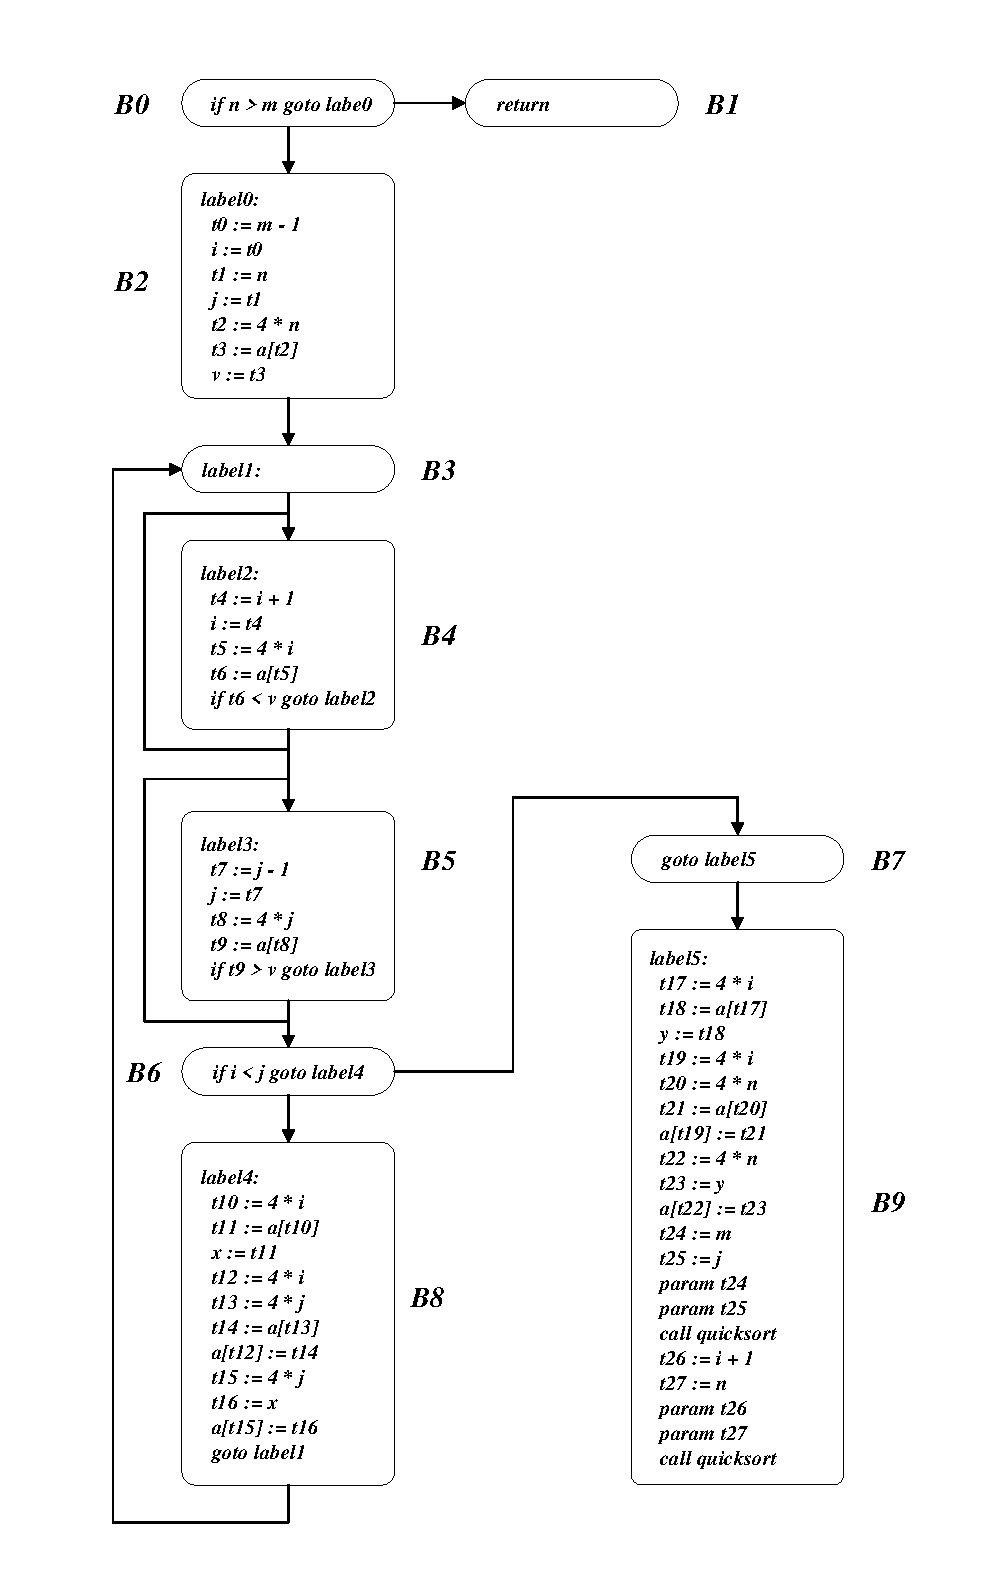
\includegraphics[width=1.01\linewidth,height=1.75\linewidth]{quicksort.eps}
%%\end{latexonly}
\caption{basic blocks of {\tt{quicksort}}}
\label{optimize_e002}
\end{center}
\end{figure}
It is possible that there are medium varialbes which is alive beyond
basic blocks in \ref{optimize_e004}. But as far as this code, there is
no any medium variable which is alive beyond basic block.
This fact is led by bellow algorithm.

Let $in[B]$ denote set of alive variables in the entrance of
basic block $B$. Samely, let $out[B]$ denote set of alive
variables in an exit of basic block $B$. Let $def[B]$ denote
set of variables which is defined before usage in basic
block $B$ and let $use[B]$ denote set of variables which is used before
definition. As described in bibliography \cite{doragon} expression
(10.11), the folloing equations holds.
\begin{eqnarray*}
out[B] & = & \bigcup_{F {\tt{\,\,follows\,\,} B}} in[F] \\
in[B]  & = & use[B] \cup (out[B] - def[B])
\end{eqnarray*}
Now our aim is to get $out$, and repeat method 
is available for solve these equations as described in bibliography
\cite{doragon}.

First, for each basic block in figure \ref{optimize_e002},
calcurate $def, use$. They become like bellow.

\vspace{0.5cm}

\begin{tabular}{|l|l|l|} \hline
   & $def$             & $use$     \\ \hline
B0 &                   & m n       \\ \hline
B1 &                   &           \\ \hline
B2 & v i j t0 t1 t2 t3 & a m n 1 4 \\ \hline
B3 &                   &           \\ \hline
B4 & t4 t5 t6          & a v i 1 4 \\ \hline
B5 & t7 t8 t9          & a v j 1 4 \\ \hline
B6 &                   & i j       \\ \hline
B7 &                   &           \\ \hline
B8 & x t10 t11 t12 t13 t14 t15 t16 & a i j 4 \\ \hline
B9 & y t17 t18 t20 t19 t21 t22 t23 & quicksort a m n \\
   & t24 t25                & i j 4 \\ \hline
B10 & t26 t27 & quicksort n i 1 \\ \hline
\end{tabular}

\vspace{0.5cm}

Generally, global variables are alive in every basic block, so
add them into every $out[B]$.

For each $B$, make $in[B]$ an empty set and 
start repeat method.

\vspace{0.5cm}

\begin{tabular}{|l|l|l|} \hline
step 0  & $out$             & $in$      \\ \hline
B0 & quicksort a 1 4   & quicksort a 1 4 m n \\ \hline
B1 & quicksort a 1 4   & quicksort a 1 4     \\ \hline
B2 & quicksort a 1 4   & quicksort a 1 4 m n \\ \hline
B3 & quicksort a 1 4   & quicksort a 1 4     \\ \hline
B4 & quicksort a 1 4   & quicksort a 1 4 v i \\ \hline
B5 & quicksort a 1 4   & quicksort a 1 4 v j \\ \hline
B6 & quicksort a 1 4   & quicksort a 1 4 i j \\ \hline
B7 & quicksort a 1 4   & quicksort a 1 4     \\ \hline
B8 & quicksort a 1 4   & quicksort a 1 4 i j \\ \hline
B9 & quicksort a 1 4 \hspace{1.7cm}
 & quicksort a 1 4 m n i j  \hspace{0.1cm} \\ \hline
\end{tabular}

\begin{tabular}{|l|l|l|} \hline
step 1  & $out$             & $in$      \\ \hline
B0 & quicksort a 1 4 m n     & quicksort a 1 4 m n   \\ \hline
B1 & quicksort a 1 4 m n     & quicksort a 1 4 m n   \\ \hline
B2 & quicksort a 1 4         & quicksort a 1 4 m n   \\ \hline
B3 & quicksort a 1 4 v i     & quicksort a 1 4 v i j \\ \hline
B4 & quicksort a 1 4 v i j   & quicksort a 1 4 v i j \\ \hline
B5 & quicksort a 1 4 v i j   & quicksort a 1 4 v i j \\ \hline
B6 & quicksort a 1 4 i j     & quicksort a 1 4 i j   \\ \hline
B7 & quicksort a 1 4 m n i j & quicksort a 1 4 m n i j  \\ \hline
B8 & quicksort a 1 4 v i     & quicksort a 1 4 v i j  \\ \hline
B9 & quicksort a 1 4  \hspace{1.7cm}
   & quicksort a 1 4 m n i j  \hspace{0.1cm} \\ \hline
\end{tabular}

\begin{tabular}{|l|l|l|} \hline
step 2  & $out$             & $in$      \\ \hline
B0 & quicksort a 1 4 m n       & quicksort a 1 4 m n        \\ \hline
B1 & quicksort a 1 4 m n       & quicksort a 1 4 m n        \\ \hline
B2 & quicksort a 1 4 v i       & quicksort a 1 4 m n        \\ \hline
B3 & quicksort a 1 4 v i j     & quicksort a 1 4 v i j      \\ \hline
B4 & quicksort a 1 4 v i j     & quicksort a 1 4 v i j      \\ \hline
B5 & quicksort a 1 4 v i j     & quicksort a 1 4 v i j      \\ \hline
B6 & quicksort a 1 4 v m n i j & quicksort a 1 4 v m n i j  \\ \hline
B7 & quicksort a 1 4 m n i j   & quicksort a 1 4 m n i j  \\ \hline
B8 & quicksort a 1 4 v i j     & quicksort a 1 4 v i j  \\ \hline
B9 & quicksort a 1 4           & quicksort a 1 4 m n i j \\ \hline
\end{tabular}

\begin{tabular}{|l|l|l|} \hline
step 3  & $out$             & $in$      \\ \hline
B0 & quicksort a 1 4 m n       & quicksort a 1 4 m n        \\ \hline
B1 & quicksort a 1 4 m n       & quicksort a 1 4 m n        \\ \hline
B2 & quicksort a 1 4 v i j     & quicksort a 1 4 m n        \\ \hline
B3 & quicksort a 1 4 v i j     & quicksort a 1 4 v i j      \\ \hline
B4 & quicksort a 1 4 v i j     & quicksort a 1 4 v i j      \\ \hline
B5 & quicksort a 1 4 v m n i j & quicksort a 1 4 v m n i j  \\ \hline
B6 & quicksort a 1 4 v m n i j & quicksort a 1 4 v m n i j  \\ \hline
B7 & quicksort a 1 4 m n i j   & quicksort a 1 4 m n i j  \\ \hline
B8 & quicksort a 1 4 v i j     & quicksort a 1 4 v i j  \\ \hline
B9 & quicksort a 1 4           & quicksort a 1 4 m n i j \\ \hline
\end{tabular}

\begin{tabular}{|l|l|l|} \hline
step 4  & $out$             & $in$      \\ \hline
B0 & quicksort a 1 4 m n       & quicksort a 1 4 m n        \\ \hline
B1 & quicksort a 1 4 m n       & quicksort a 1 4 m n        \\ \hline
B2 & quicksort a 1 4 v i j     & quicksort a 1 4 m n        \\ \hline
B3 & quicksort a 1 4 v i j     & quicksort a 1 4 v i j      \\ \hline
B4 & quicksort a 1 4 v m n i j & quicksort a 1 4 v m n i j  \\ \hline
B5 & quicksort a 1 4 v m n i j & quicksort a 1 4 v m n i j  \\ \hline
B6 & quicksort a 1 4 v m n i j & quicksort a 1 4 v m n i j  \\ \hline
B7 & quicksort a 1 4 m n i j   & quicksort a 1 4 m n i j  \\ \hline
B8 & quicksort a 1 4 v i j     & quicksort a 1 4 v i j  \\ \hline
B9 & quicksort a 1 4           & quicksort a 1 4 m n i j \\ \hline
\end{tabular}

\begin{tabular}{|l|l|l|} \hline
step 5  & $out$             & $in$      \\ \hline
B0 & quicksort a 1 4 m n       & quicksort a 1 4 m n        \\ \hline
B1 & quicksort a 1 4 m n       & quicksort a 1 4 m n        \\ \hline
B2 & quicksort a 1 4 v i j     & quicksort a 1 4 m n        \\ \hline
B3 & quicksort a 1 4 v m n i j & quicksort a 1 4 v m n i j  \\ \hline
B4 & quicksort a 1 4 v m n i j & quicksort a 1 4 v m n i j  \\ \hline
B5 & quicksort a 1 4 v m n i j & quicksort a 1 4 v m n i j  \\ \hline
B6 & quicksort a 1 4 v m n i j & quicksort a 1 4 v m n i j  \\ \hline
B7 & quicksort a 1 4 m n i j   & quicksort a 1 4 m n i j  \\ \hline
B8 & quicksort a 1 4 v m n i j & quicksort a 1 4 v m n i j  \\ \hline
B9 & quicksort a 1 4           & quicksort a 1 4 m n i j \\ \hline
\end{tabular}

\begin{tabular}{|l|l|l|} \hline
step 6  & $out$             & $in$      \\ \hline
B0 & quicksort a 1 4 m n       & quicksort a 1 4 m n        \\ \hline
B1 & quicksort a 1 4 m n       & quicksort a 1 4 m n        \\ \hline
B2 & quicksort a 1 4 v i j     & quicksort a 1 4 m n        \\ \hline
B3 & quicksort a 1 4 v m n i j & quicksort a 1 4 v m n i j  \\ \hline
B4 & quicksort a 1 4 v m n i j & quicksort a 1 4 v m n i j  \\ \hline
B5 & quicksort a 1 4 v m n i j & quicksort a 1 4 v m n i j  \\ \hline
B6 & quicksort a 1 4 v m n i j & quicksort a 1 4 v m n i j  \\ \hline
B7 & quicksort a 1 4 m n i j   & quicksort a 1 4 m n i j  \\ \hline
B8 & quicksort a 1 4 v m n i j & quicksort a 1 4 v m n i j  \\ \hline
B9 & quicksort a 1 4           & quicksort a 1 4 m n i j \\ \hline
\end{tabular}

\vspace{0.5cm}
For each basic block $B$, $in[B]$ of step 5 is equal to that of step 6.
So the repeat method is finished.

For each basic block $B$ in figure \ref{optimize_e002},
$out[B]$ becomes like bellow.

\vspace{0.5cm}

\begin{tabular}{|l|l|l|} \hline
   & $out$                            \\ \hline
B0 & quicksort a m n  1 4             \\  \hline
B1 & quicksort a 1 4                  \\ \hline
B2 & quicksort a m n  v i j 1 4       \\ \hline
B3 & quicksort a m n  v i j 1 4       \\ \hline
B4 & quicksort a m n  v i j 1 4       \\ \hline
B5 & quicksort a m n  v i j 1 4       \\ \hline
B6 & quicksort a m n  v i j 1 4       \\ \hline
B7 & quicksort a m n    i j 1 4       \\ \hline
B8 & quicksort a m n  v i j 1 4       \\ \hline
B9 & quicksort a 1 4              \\ \hline
\end{tabular}

\vspace{0.5cm}

Similally, for figure \ref{optimize_e001},
this algorithm tell us that
`{\tt{t0}}' and `{\tt{t1}}'
are in $out[B]$ for every basic block $B$, except for last basic block.

\subsection{Assignment and common expression}
\label{optimize_e_assign}
We've discussed about how to devide into basic block
and how to analize alive variable until previous section. Now here, 
we'll think about how to detect redundant assignment and common
expression from 3 address codes.

We'll express basic block with {\em dag} described in bibliography
 \cite{doragon}. {\em dag} is like bellow structure.

\begin{verbatim}
struct dag {  // Node of dag
  tac* m_tac;        // Correspond 3 address code. Label of this node.
  vector<var*> m_vars;      // Calcurating variables. Identifier list.
  vector<dag*> m_parents;   // Parent
  dag* m_left;              // Left child
  dag* m_right;             // Right child
  dag* m_extra;             // 3rd child for `x' of x[y] := z
  static vector<dag*> all;  // All list
  dag() : m_tac(0), m_left(0), m_right(0) { all.push_back(this); }
};

map<var*, dag*> node;  // Table from variable to node.
\end{verbatim}

Before showing conversion from basic block to {\em dag},
or corresponding code generation algorithm,
let's think about bellow simple example.

\begin{Example}
\label{optimize_e006}
\begin{verbatim}
int n; void f(void){ ++n; }
\end{verbatim}
3 address codes become like bellow.
\begin{verbatim}
f:
   n := n + 1
  t0 := n
\end{verbatim}
Figure \ref{optimize_e005} illustrates
process of creating {\em dag} from these 3 address codes.
\begin{figure}[htbp]
\begin{center}
%%\begin{htmlonly}
%%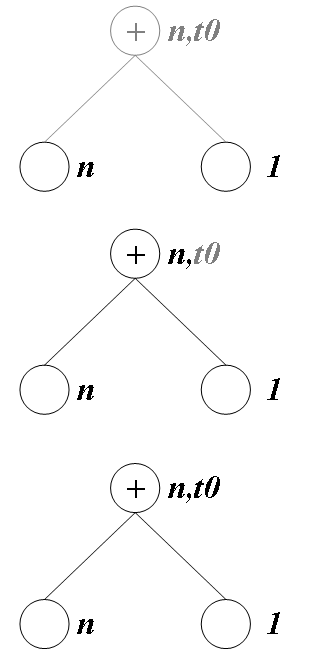
\includegraphics[width=0.5\linewidth,height=1.01\linewidth]{opt000.png}
%%\end{htmlonly}
%%\begin{latexonly}
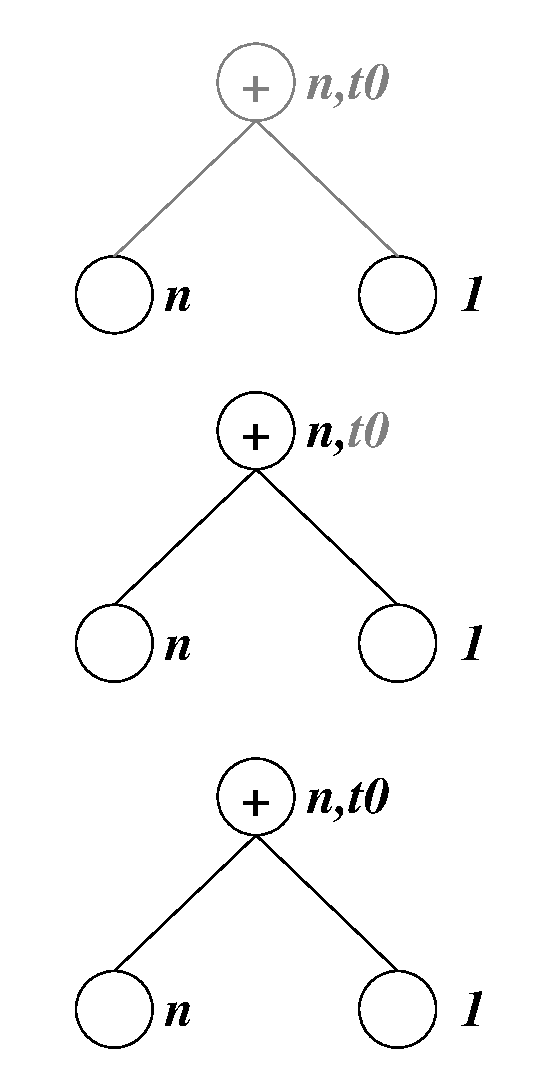
\includegraphics[width=0.5\linewidth,height=1.01\linewidth]{opt000.eps}
%%\end{latexonly}
\caption{{\em dag} of example \ref{optimize_e006}}
\label{optimize_e005}
\end{center}
\end{figure}

\begin{enumerate}
\item At {\tt{n := n + 1}}, for right hand `{\tt{n}}', 
{\tt{node[n]}} is not defined, so create new node. And
add `{\tt{n}}' into identifier list {\tt{m\_vars}}.
Finally make this {\tt{dag}} {\tt{node[n]}}.

\item At {\tt{n := n + 1}}, for `{\tt{1}}' ,
 {\tt{node[1]}} is not defioned, so create new node. And 
add `{\tt{1}}' into identifier list {\tt{m\_vars}}.
Finally make this {\tt{dag}} {\tt{node[1]}}.

\item From {\tt{dag::all}}, find the node whose label is `{\tt{+}}'
and whose left child is equal to {\tt{node[n]}}
and whose right child is equal to {\tt{node[1]}}.
There is not such a node, so create {\tt{dag}}  and
make it satisfying the condition.
And make this {\tt{dag}} {\tt{node[n]}}.

\item At {\tt{t0 := n}}, for `{\tt{n}}',
{\tt{node[n]}} is already defined.
Add `{\tt{t0}}' into identifier list {\tt{m\_vars}} of {\tt{node[n]}}.
\end{enumerate}
After constructing {\em dag}, generate 3 address codes by evaluating
in order.

\begin{enumerate}
\item Evaluate the node whose identifier list is `{\tt{n}}'.
      Here no code is generated. The result is `{\tt{n}}'.

\item Evaluate the node whose identifier list is `{\tt{1}}'.
      Here no code is generated. The result is `{\tt{1}}'.

\item Evaluate the node whose identifier list is `{\tt{n, t0}}'.
      Find identifer $x$ from identifier list, where {\tt{node[$x$]}} is equal
      to this node and $x$ is alive in an exit of basic block.
      Here we chose `{\tt{n}}'.
      And generate code {\tt{n := n + 1}}.
 
\item For the other element of identifier list, if the identifier
      is alive in an eit of basic block, generate assignment code.
      In this case, {\tt{t0}} is not alive in an exit of this
      basic block.

\end{enumerate}
At last, {\tt{n := n + 1}} is only generated.
\end{Example}

We can get {\em dag} of basic block by bellow algorithm.

\begin{quote}
{\bf Creation {\em dag} of basic block algorithm}

For each 3 address code of basic block, apply bellow. 
\begin{enumerate}
\item For {\tt{x := y $op$ z}}, if {\tt{y}} is not specified,
      the 3 address code is special like 
      return without return value
      ({\tt{return3ac::y}} is 0),
      unconditional jump ({\tt{goto3ac::y}} is 0),
      label ({\tt{to3ac}}) or
      assembly output({\tt{asm3ac}}).
      In this case, create new node and terminate this procedure. 

\item If {\tt{node[y]}} is not still defined, 
      create new node and add {\tt{y}} into its {\tt{m\_vars}}.
      Make this dag {\tt{node[y]}}. 

\item If {\tt{z}} is specified and {\tt{node[z]}} is not still defined,
      create new node and add {\tt{z}} into its {\tt{m\_vars}}.
      Make this dag {\tt{node[z]}}.

\item 
\label{optimize_e047}
Get node $n$ like bellow.

\begin{enumerate}
\item If the 3 address code is {\tt{x := y}},
      let {\tt{node[y]}} to be $n$.
\item If the 3 address code is {\tt{call}} or {\tt{va\_arg}},
      create new node and let it to be $n$.
\item For {\tt{x := y $op$ z}}, if {\tt{x}} is not specified,
      create new node and let it to be $n$.
\item For 3 address code {\tt{x := y $op$ z}} expcet for above,
      find from {\tt{dag::all}} the node 
      whose left child is {\tt{node[y]}},
      whose right child is {\tt{node[z]}}
      and
      whose label is $op$. Especially,
\begin{enumerate}
\item In case of {\tt{x := y[z]}}, {\tt{x := *y}},
      type of {\tt{x}} must be {\it
      compatible}.
\item In case of {\tt{x[y] := z}}, {\tt{alloca x, y}},
      {\tt{x}} must be equal.
\item In case of {\tt{x := (type)y}}, {\tt{type}} must be
     {\it compatible}.
\end{enumerate}
      If exists, let it to be $n$.
\item \label{optimize_e109}
      If there is not such a node and in case of {\tt{x := y[z]}},
      find from {\tt{dag::all}} the node like bellow.
      \begin{itemize}
      \item label is {\tt{x'[y'] := z'}}.
      \item {\tt{node[y]}} is equal to the node.
      \item {\tt{node[z]}} is equal to left child of the node.
      \item type of {\tt{x}} is {\it compatible} with that of {\tt{z'}}.
      \end{itemize}
      If exists, let its right child to be $n$.
\item \label{optimize_e064}
If there is not such a node, create new node and let it to be $n$.
For {\tt{x[y] := z}}, if {\tt{node[x]}} already exists, let {\tt{node[x]}}
to be 3rd child of $n$.
\end{enumerate}
\item \label{optimize_e112}
      If this 3 address code is {\tt{call3ac} or {\tt{invladdr3ac}}},
      apply bellow and terminate this procedure.
      \begin{enumerate}
      \item If this 3 address code is {\tt{x := call f}} and {\tt{x}} 
            is not 0, add {\tt{x}} into {\tt{m\_vars}} of $n$ and
            update {\tt{node[x]}} to be $n$. 
      \item Apply {\bf Code generation algorithm from {\em dag}}
	    described bellow.
      \item Clear {\tt{node}}.
      \item Clear {\tt{result}} described bellow.
      \end{enumerate}

\item For 3 address code {\tt{x := y $op$ z}}, if {\tt{x}} is not specified,
      terminate this procedure.

\item Add {\tt{x}} of 3 address code {\tt{x := y op z}} into
      {\tt{m\_vars}} of $n$ which is gotten in \ref{optimize_e047}.
      And update {\tt{node[x]}} to be $n$. 
\end{enumerate}

\end{quote}

For generating code from {\em dag}, apply bellow.

\begin{quote}
{\bf Code generation algorithm from {\em dag}}

For each node of {\tt{dag::all}}, apply bellow procedure which returns
{\tt{var*}}. And keep the result of this procedure in
{\tt{map<dag*, var*> result}}.

\begin{enumerate}
\item If the label of the node is none, call bellow procedure
      {\bf Assignment judge algorithm} and return it.

\item \label{optimize_e048}
      Let {\tt{x := y $op$ z}} denote the label.
      For the left child $\ell$, replace `{\tt{y}}' with
      {\tt{result[$\ell$]}}.
\item \label{optimize_e049}
      Simillary, for the right child $r$, replace `{\tt{z}}'
      with {\tt{result[$r$]}}.
\item \label{optimize_e050}
      Copy the 3 address code {\tt{x := y $op$ z}} to the container
      for optimization result, where {\tt{y}} and {\tt{z}}
      is obtained in \ref{optimize_e048}, \ref{optimize_e049}.
\item Update `{\tt{x}}' of {x := y $op$ z} which is copied in
      \ref{optimize_e050} appling bellow procedure
      {\bf Assignment judge algorithm}. Now we'll refere updated
       {\tt{x}} as just `{\tt{x}}'.
\item  If `{\tt{x}}' is zero or this node has a parent or parents,
       return `{\tt{x}}'.
\item If `{\tt{x}}' is alive in an exit of this basic block,
      return `{\tt{x}}'.
\item If `{\tt{x}}' is used before it is defined
      in this basic block, and {\tt{node[x]}} is equal to
      the current {\tt{dag}}, return `{\tt{x}}'.
\item For `{\tt{x}}', if there exists a 3 address code {\tt{p := \&x}} in this
      basic block, return `{\tt{x}}'.
\item \label{optimize_e057}
      If a 3 address code copied at \ref{optimize_e050} is
      {\tt{x := call y}} and `{\tt{x}}' is used before it is
      defined, change it {\tt{call y}} and return {\tt{0}}.
\item If a 3 address code copied at \ref{optimize_e050} is
      {\tt{alloca x, y}}, return {\tt{x}}.
\item If a 3 address code copied at \ref{optimize_e050} is
      {\tt{x[y] := z}} and there exists one like bellow
      at identifier list of {\tt{node[x]}}:
      \begin{enumerate}
      \item Alive in an exit of this this basic block
      \item Used before defined at this basic block
      \end{enumerate}
      then, return {\tt{x}}.
\item \label{optimize_e056}
      Erase a 3 address code copied at \ref{optimize_e050} 
      from the container for optimization result.
\item return {\tt{0}}.
\end{enumerate}
\end{quote}

\begin{quote}
{\bf Assignment judge algorithm}

\begin{enumerate}
\item If the identifier list {\tt{m\_vars}} of this node is empty,
      return {\tt{0}}.
\item  \label{optimize_e067}
      If the condition of
      {\bf Assignment judge algorithm (Special case) }
      described bellow holds true, return the result.
\item \label{optimize_e055}
      If this node is leaf, 
      let the 1st elemnt of the identifier list to be `{\tt{y}}'.
\item If the label is {\tt{loff}} of this node,
      let the 1st elemnt of the identifier list to be `{\tt{y}}'.
\item \label{optimize_e054}
      Otherwise,
      find from the identifier list in the order described bellow:
      \begin{enumerate}
      \item Alive in an exit of this this basic block
      \item Used before defined at this basic block
      \item `{\tt{y}}' where {\tt{node[y]}} is equal to this node
      \item Address is referenced at this basic block
      \end{enumerate}
      If not exists, let the 1st elemnt of the identifier list to be `{\tt{y}}'.
 \item 
      For each element `{\tt{x}}' of identfier list which follows `{\tt{y}}',
      apply bellow.
\begin{enumerate}
\item If label of this node is {\tt{loff}},  generate {\tt{x := y}}.
\item \label{optimize_e052}
      If the label of parent of this node is a 3 address code
      {\tt{p := \&x}} and this node is leaf, generate {\tt{x := y}}.
\item If there exists parent `{\tt{p}}' of this node which satisfies
      bellow condition, generate {\tt{x := y}}:
      \begin{enumerate}
      \item label of `{\tt{p}}' is {\tt{loff}}
      \item `{\tt{p}}' has 3rd child.
      \item `{\tt{x}}' exists in identifier list of 3rd child of `{\tt{p}}'
      \end{enumerate}
\item If {\tt{node[x]}} is not equal to this node, 
      not generate assignment.
\item \label{optimize_e053} 
      If `{\tt{x}}' is alive in an exit of this basic block,
      generate {\tt{x := y}}.
\item \label{optimize_e110} 
      If there exists a 3 address code {\tt{p := \&x}} in this
      basic block, generate {\tt{x := y}}
      (\ref{optimize_e111} distinguishes this and \ref{optimize_e052}).
\item If `{\tt{x}}' is used before it is defined, 
      generate {\tt{x := y}}.
\end{enumerate}

\item \label{optimize_e111}
If the contition of \ref{optimize_e052} holds true,
      return `{\tt{x}}'. Otherwise return `{\tt{y}}'. 
\end{enumerate}
\end{quote}

\begin{quote}
{\bf Assignment judge algorithm (Special case) }
\begin{enumerate}
\item \label{optimize_e072}
      Find from {\tt{m\_vars}} the identifier `{\tt{t}}' where
      {\tt{node[t]}} is equal to this node. If not, it's not special so
      return {\tt{0}}.
\item If `{\tt{t}}' is the 1st element of {\tt{m\_vars}} at
      \ref{optimize_e072}, it's not special so return {\tt{0}}.

\item For the 1st element `{\tt{x}}' of {\tt{m\_vars}},
      generate {\tt{t := x}}.

\item Return `{\tt{t}}'.
\end{enumerate}
\end{quote}

We'll think about and investigate how these algorithm work for some examples.

\begin{Example}
\label{optimize_e007}
\begin{verbatim}
int n; void f(int a, int b, int c){ n = a + b + c; }
\end{verbatim}
3 address codes become like bellow.
\begin{verbatim}
f:
  t0 := a + b
  t1 := t0 + c
   n := t1
\end{verbatim}
Figure \ref{optimize_e008} illustrates the process of creating
{\em dag} from these 3 address codes.
\begin{figure}[htbp]
\begin{center}
%%\begin{htmlonly}
%%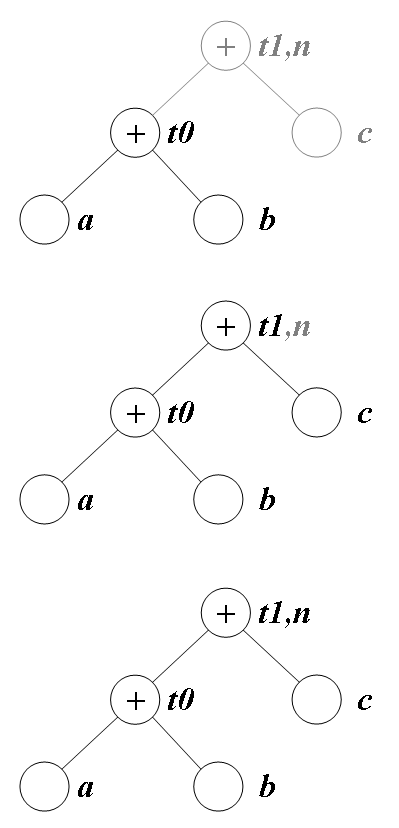
\includegraphics[width=0.468\linewidth,height=1.0\linewidth]{opt001.png}
%%\end{htmlonly}
%%\begin{latexonly}
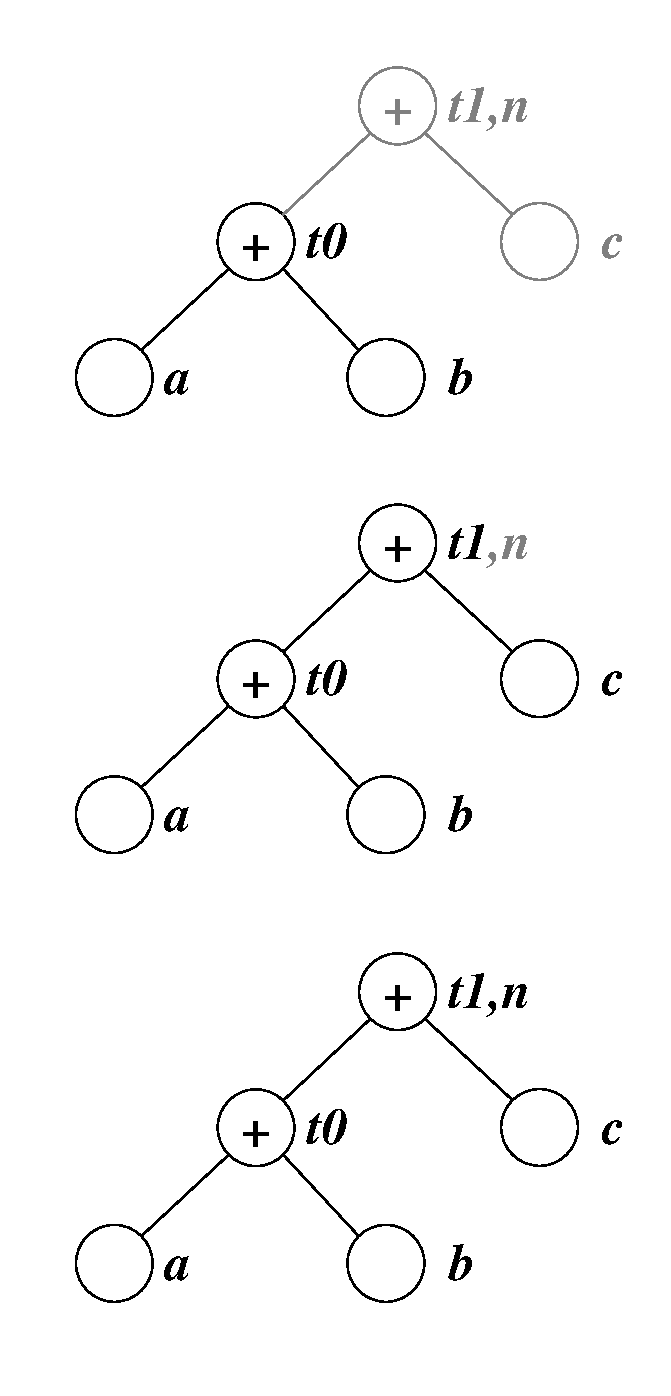
\includegraphics[width=0.468\linewidth,height=1.0\linewidth]{opt001.eps}
%%\end{latexonly}
\caption{{\em dag} of example \ref{optimize_e007}}
\label{optimize_e008}
\end{center}
\end{figure}
Function `{\tt{f}}' is consist of one basic block, and 
`{\tt{n}}' is alive in an exit of this basic block.
For the node whose identifier list is `{\tt{t1, n}}',
chose `{\tt{n}}' at \ref{optimize_e054} of {\bf Assignment judge algorithm}.
After appling algorithms of this section,
3 address codes become like bellow.
\begin{verbatim}
f:
  t0 := a + b
   n := t0 + c
\end{verbatim}
\end{Example}

\begin{Example}
\label{optimize_e009}
\begin{verbatim}
int f(void){ int n = 2; return n + 3; }
\end{verbatim}
3 address codes become like bellow.
\begin{verbatim}
f:
   n := 2
  t0 := n + 3
   return t0
\end{verbatim}
Figure \ref{optimize_e010} illustrates the process of creating
{\em dag} from these 3 address codes.
\begin{figure}[htbp]
\begin{center}
%%\begin{htmlonly}
%%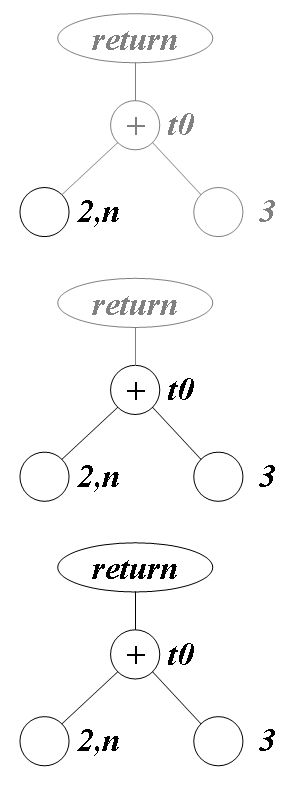
\includegraphics[width=0.392\linewidth,height=1.0\linewidth]{opt002.png}
%%\end{htmlonly}
%%\begin{latexonly}
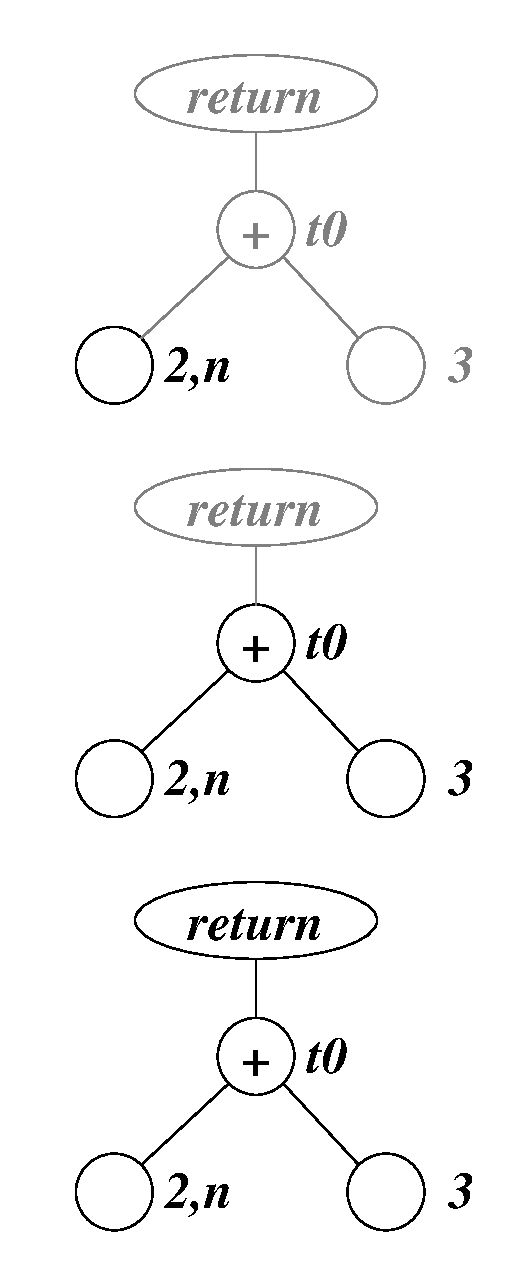
\includegraphics[width=0.392\linewidth,height=1.0\linewidth]{opt002.eps}
%%\end{latexonly}
\caption{{\em dag} of example \ref{optimize_e009}}
\label{optimize_e010}
\end{center}
\end{figure}
Function `{\tt{f}}' is consist of one basic block, and 
`{\tt{2, 3}}' are alive in an exit of this basic block.
For the node whose identifier list is `{\tt{2, n}}',
chose `{\tt{2}}' at \ref{optimize_e055} of {\bf Assignment judge algorithm}.
After appling algorithms of this section,
3 address codes become like bellow.
\begin{verbatim}
f:
  t0 := 2 + 3
   return t0
\end{verbatim}
This example shows that
compile-time evaluationable 3 address code may be generated
after appling algorithms of this section. But in this section,
no more discussion.
\end{Example}

\begin{Example}
\label{optimize_e011}
\begin{verbatim}
int n; void g(void); void f(void){ n = 2; g(); ++n; }
\end{verbatim}
3 address codes become like bellow.
\begin{verbatim}
f:
   n := 2
  t0 := 2
   call g
   n := n + 1
  t1 := n
\end{verbatim}
Figure \ref{optimize_e012} illustrates the process of creating
{\em dag} at the point that {\tt{call g}} is processed.

\begin{figure}[htbp]
\begin{center}
%%\begin{htmlonly}
%%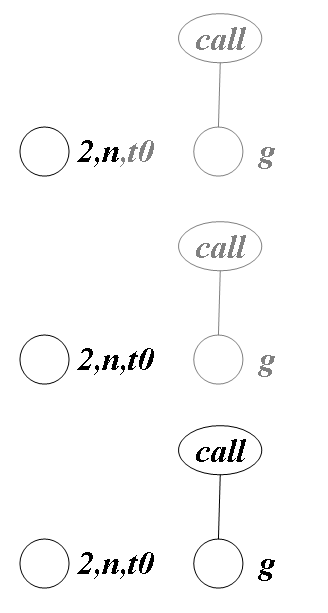
\includegraphics[width=0.530\linewidth,height=1.0\linewidth]{opt003.png}
%%\end{htmlonly}
%%\begin{latexonly}
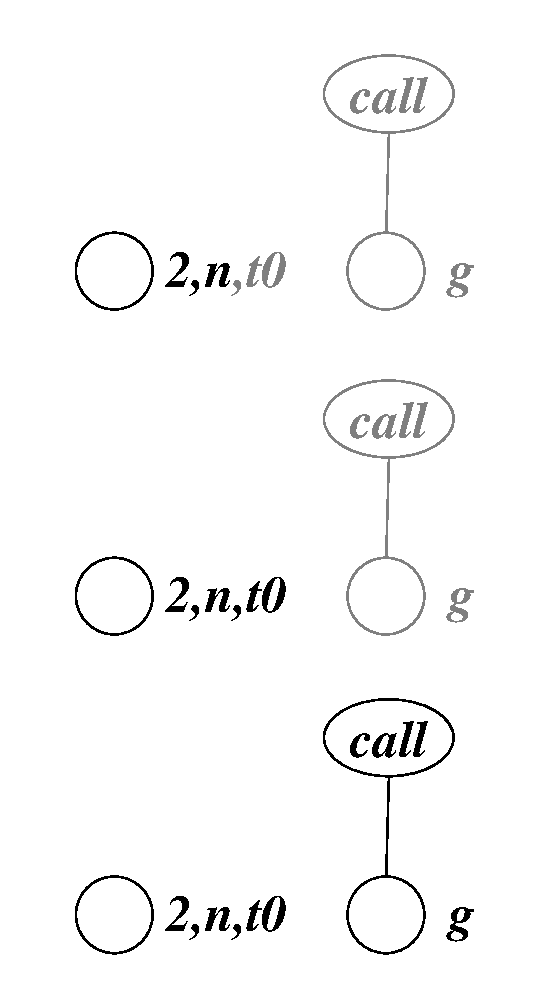
\includegraphics[width=0.530\linewidth,height=1.0\linewidth]{opt003.eps}
%%\end{latexonly}
\caption{{\em dag} of example \ref{optimize_e011}}
\label{optimize_e012}
\end{center}
\end{figure}
Function `{\tt{f}}' is consist of one basic block, and 
`{\tt{n, g, 1, 2}}' are alive in an exit of this basic block.
At \ref{optimize_e112} of {\bf Creation {\em dag} of basic block algorithm},
for {\tt{call g}},
{\bf Code generation algorithm from {\em dag}} is applied.
For the node whose identifier list is `{\tt{2, n, t0}}',
chose `{\tt{2}}'
at \ref{optimize_e055} of {\bf Assignment judge algorithm}.
{\tt{n := 2}} is generated, but for `{\tt{t0}}', 
assignment isn't generated. 
After appling algorithms of this section,
This {\em dag} is converted to like bellow.
\begin{verbatim}
   n := 2
   call g
\end{verbatim}
\end{Example}

\begin{Example}
\label{optimize_e013}
\begin{verbatim}
int n; void f(int* p){ n = 2; *p = 3; ++n; }
\end{verbatim}
3 address codes become like bellow.
\begin{verbatim}
f:
   n := 2
  t0 := 2
  t1 := p
 *t1 := 3
  t2 := 3
   n := n + 1
  t3 := n
\end{verbatim}
Figure \ref{optimize_e014} illustrates the process of creating
{\em dag} at the point that {\tt{*t1 := 3}} is processed.
\begin{figure}[htbp]
\begin{center}
%%\begin{htmlonly}
%%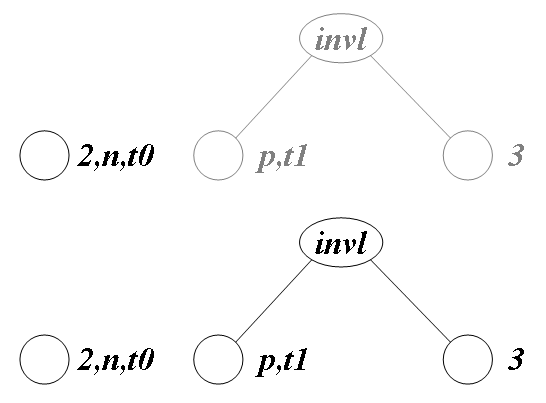
\includegraphics[width=1.0\linewidth,height=0.729\linewidth]{opt004.png}
%%\end{htmlonly}
%%\begin{latexonly}
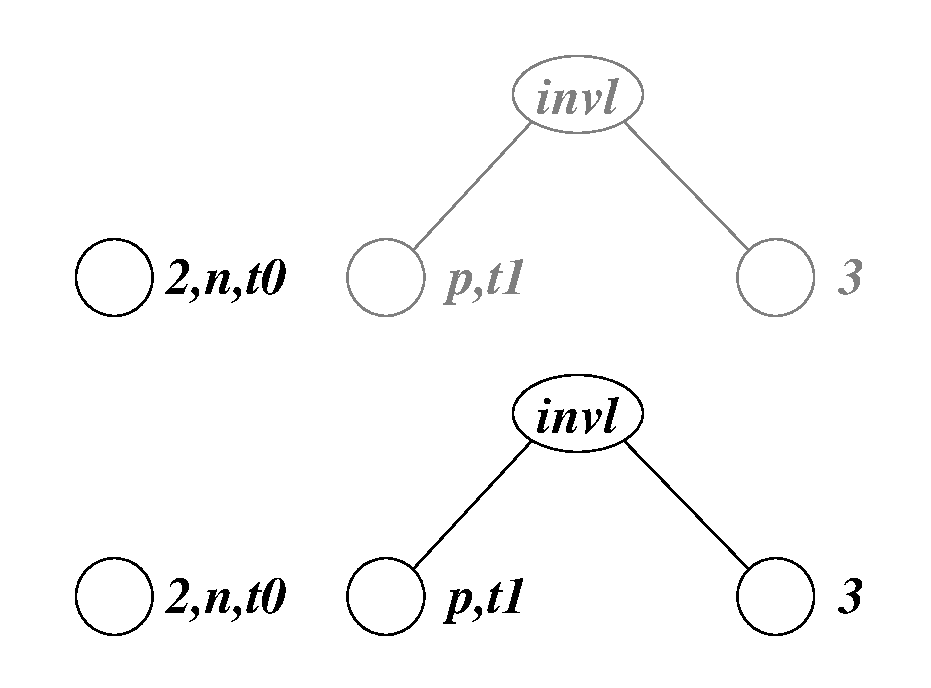
\includegraphics[width=1.0\linewidth,height=0.729\linewidth]{opt004.eps}
%%\end{latexonly}
\caption{{\em dag} of example \ref{optimize_e013}}
\label{optimize_e014}
\end{center}
\end{figure}

Function `{\tt{f}}' is consist of one basic block, and 
`{\tt{n, 1, 2, 3}}' are alive in an exit of this basic block.
At \ref{optimize_e112} of {\bf Creation {\em dag} of basic block algorithm},
for {\tt{*t1 := 3}},
{\bf Code generation algorithm from {\em dag}} is applied.
For the node whose identifier list is `{\tt{2, n, t0}}',
chose `{\tt{2}}'
at \ref{optimize_e055} of {\bf Assignment judge algorithm}.
{\tt{n := 2}} is generated, but for `{\tt{t0}}', 
assignment isn't generated.
For the node whose identifier list is `{\tt{p, t1}}',
chose `{\tt{p}}'
at \ref{optimize_e055} of {\bf Assignment judge algorithm}.
For `{\tt{t0}}', 
assignment isn't generated. 
After appling algorithms of this section,
this dag is converted to like bellow.
\begin{verbatim}
   n := 2
  *p := 3
\end{verbatim}
\end{Example}

\begin{Example}
\label{optimize_e039}
\begin{verbatim}

int f(int a, int b)
{ int c = a, d = b; return (a + b) + (c + d); }
\end{verbatim}
3 address codes become like bellow.
\begin{verbatim}
f:
  t0 := a
   c := t0
  t1 := b
   d := t1
  t2 := a + b
  t3 := c + d
  t4 := t2 + t3
  return t4
\end{verbatim}
Figure \ref{optimize_e040} shows {\em dag} for these 3 address codes.
\begin{figure}[htbp]
\begin{center}
%%\begin{htmlonly}
%%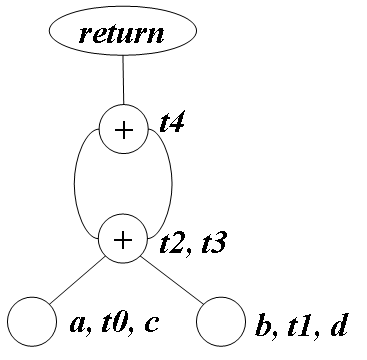
\includegraphics[width=0.724\linewidth,height=0.7\linewidth]{opt021.png}
%%\end{htmlonly}
%%\begin{latexonly}
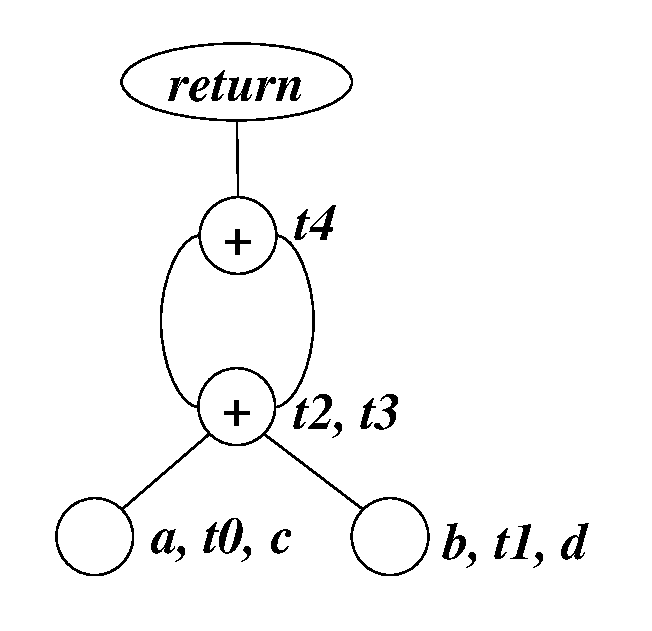
\includegraphics[width=0.724\linewidth,height=0.7\linewidth]{opt021.eps}
%%\end{latexonly}
\caption{{\em dag} of example \ref{optimize_e039}}
\label{optimize_e040}
\end{center}
\end{figure}
For the node whose identifier list is `{\tt{a, t0, c}}',
chose `{\tt{a}}' at \ref{optimize_e055} of {\bf Assignment judge algorithm}.
Assignment is not generated for `{\tt{t0, c}}'.
Simillary, for the node whose identifier list is `{\tt{b, t1, d}}',
chose `{\tt{b}}' at \ref{optimize_e055}
of {\bf Assignment judge algorithm} and
assignment is not generated for `{\tt{t1, d}}'.
For the node whose identifier list is `{\tt{t2, t3}}',
chose `{\tt{t2}}' at \ref{optimize_e054}
of {\bf Assignment judge algorithm}.
After appling algorithms of this section,
3 address codes become like bellow.
\begin{verbatim}
f:
  t2 := a + b
  t4 := t2 + t2
  return t4
\end{verbatim}
\end{Example}

\begin{Example}
\label{optimize_e041}
\begin{verbatim}

int f(int a, int b, int c, int d, int e)
{ return (a+b+(a+b-c)*(d+e))*((a+b-c)*(d+e)-e); }
\end{verbatim}
3 address codes become like bellow.
\begin{verbatim}
f:
  t0 := a + b
  t1 := a + b
  t2 := t1 - c
  t3 := d + e
  t4 := t2 * t3
  t5 := t0 + t4
  t6 := a + b
  t7 := t6 - c
  t8 := d + e
  t9 := t7 * t8
  t10 := t9 - e
  t11 := t5 * t10
  return t11
\end{verbatim}
Figure \ref{optimize_e042} shows {\em dag} for these 3 address codes.
\begin{figure}[htbp]
\begin{center}
%%\begin{htmlonly}
%%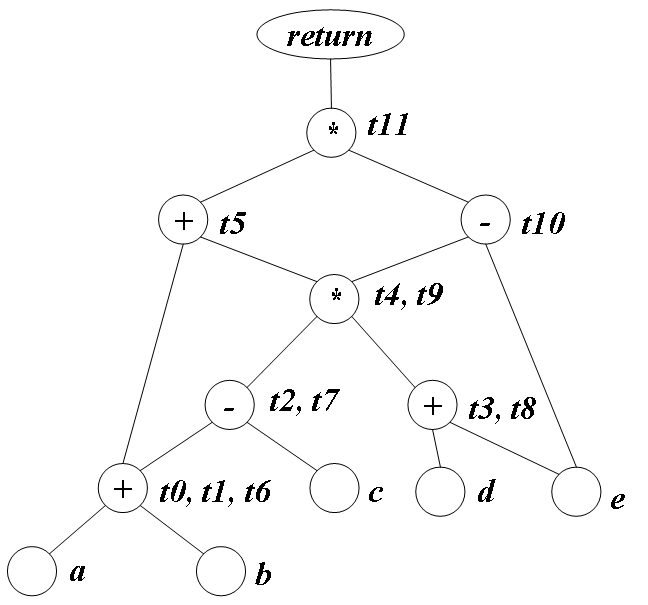
\includegraphics[width=1.051\linewidth,height=1.0\linewidth]{opt022.png}
%%\end{htmlonly}
%%\begin{latexonly}
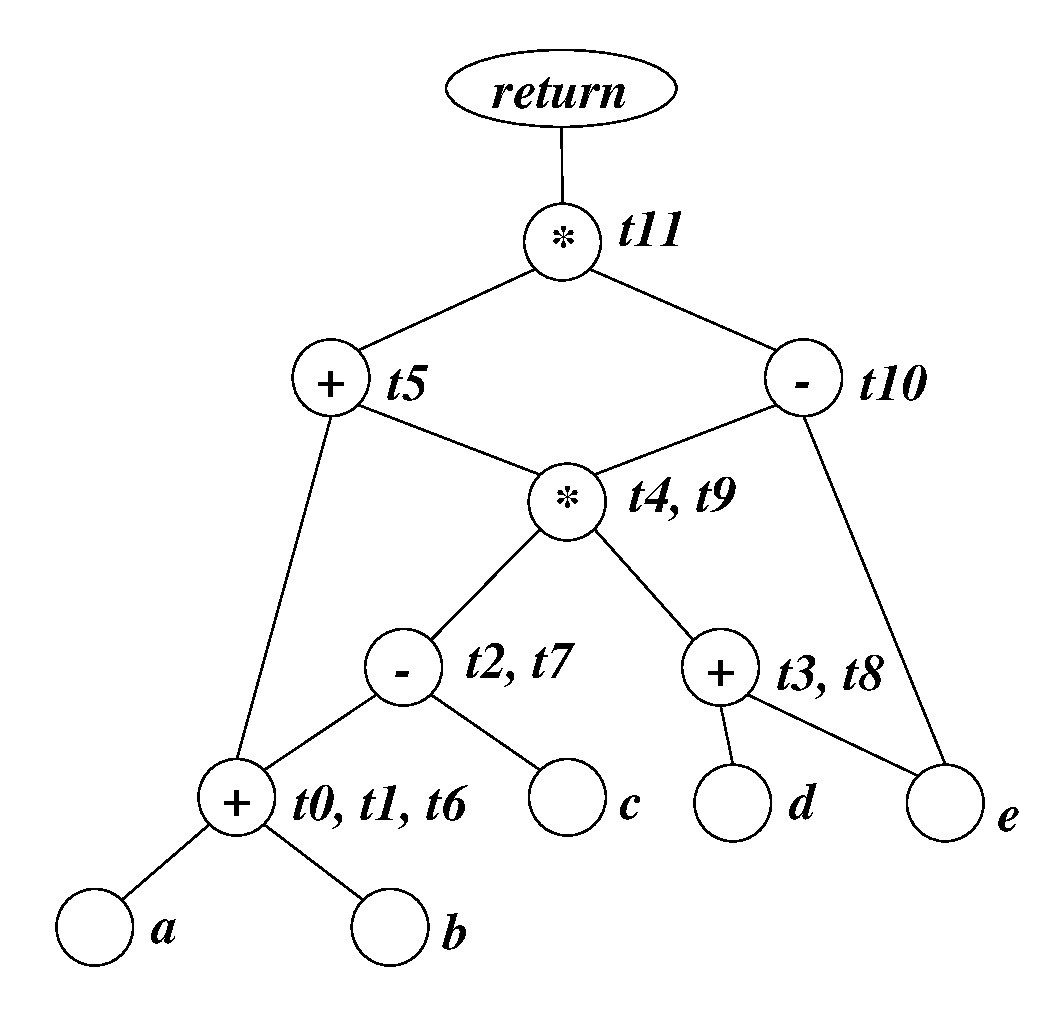
\includegraphics[width=1.051\linewidth,height=1.0\linewidth]{opt022.eps}
%%\end{latexonly}
\caption{{\em dag} of example \ref{optimize_e041}}
\label{optimize_e042}
\end{center}
\end{figure}
Function `{\tt{f}}' is consist of one basic block, and 
no identifier is alive in an exit of this basic block.
For the node whose identifier list is `{\tt{t0, t1, t6}}',
chose `{\tt{t0}}' at \ref{optimize_e054}
of {\bf Assignment judge algorithm}.
For the node whose identifier list is `{\tt{t2, t7}}',
chose `{\tt{t2}}' at \ref{optimize_e054}
of {\bf Assignment judge algorithm}.
For the node whose identifier list is `{\tt{t3, t8}}',
chose `{\tt{t3}}' at \ref{optimize_e054}
of {\bf Assignment judge algorithm}.
For the node whose identifier list is `{\tt{t4, t9}}',
chose `{\tt{t3}}' at \ref{optimize_e054}
of {\bf Assignment judge algorithm}.
After appling algorithms of this section,
3 address codes become like bellow.
\begin{verbatim}
f:
  t0 := a + b
  t2 := t0 - c
  t3 := d + e
  t4 := t2 * t3
  t5 := t0 + t4
  t10 := t4 - e
  t11 := t5 * t10
  return t11
\end{verbatim}
\end{Example}

\begin{Example}
\label{optimize_e043}
\begin{verbatim}

int x, y;
void f(int b){ int a = b + x; b = a - y; x = b + x; y = a - y; }
\end{verbatim}
3 address codes become like bellow.
\begin{verbatim}
f:
  t0 := b + x
   a := t0
  t1 := a - y
   b := t1
  t2 := b + x
   x := t2
  t3 := a - y
   y := t3
\end{verbatim}
Figure \ref{optimize_e044} shows {\em dag} for these 3 address codes.
\begin{figure}[htbp]
\begin{center}
%%\begin{htmlonly}
%%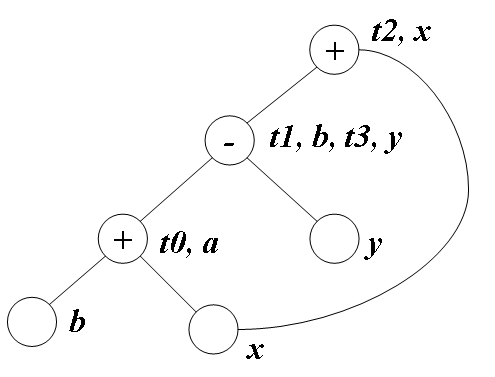
\includegraphics[width=0.7\linewidth,height=0.540\linewidth]{opt023.png}
%%\end{htmlonly}
%%\begin{latexonly}
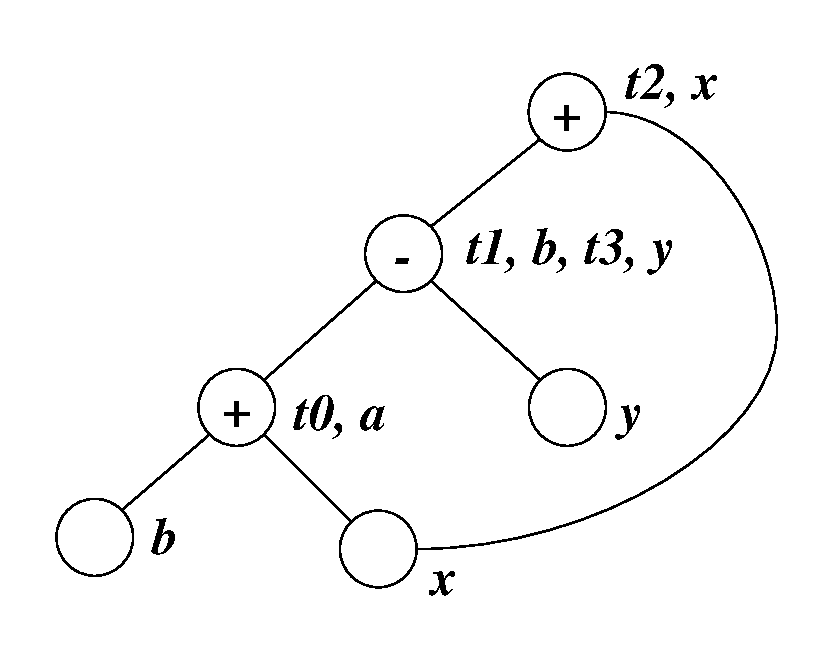
\includegraphics[width=0.7\linewidth,height=0.540\linewidth]{opt023.eps}
%%\end{latexonly}
\caption{{\em dag} of example \ref{optimize_e043}}
\label{optimize_e044}
\end{center}
\end{figure}
Function `{\tt{f}}' is consist of one basic block, and 
`{\tt{x, y}}' are alive in an exit of this basic block.
For the node whose identifier list is `{\tt{t0, a}}',
chose `{\tt{t0}}' at \ref{optimize_e054} of {\bf Assignment judge algorithm}.
For the node whose identifier list is `{\tt{t1, b, t3, y}}',
chose `{\tt{y}}' at \ref{optimize_e054} of {\bf Assignment judge algorithm}.
For the node whose identifier list is `{\tt{t2, y}}',
chose `{\tt{y}}' at \ref{optimize_e054} of {\bf Assignment judge algorithm}.
After appling algorithms of this section,
3 address codes become like bellow.
\begin{verbatim}
f:
  t0 := b + x
  y := t0 - y
  x := y + x
\end{verbatim}
\end{Example}

\begin{Example}
\label{optimize_e045}
\begin{verbatim}

int x, y;
void f(int a, int b, int c){ x = a + b; a = a - c; b = b + c; y = a + b; }
\end{verbatim}
3 address codes become like bellow.
\begin{verbatim}
f:
  t0 := a + b
   x := t0
  t1 := a - c
   a := t1
  t2 := b + c
   b := t2
  t3 := a + b
   y := t3
\end{verbatim}
Figure \ref{optimize_e046} shows {\em dag} for these 3 address codes.
\begin{figure}[htbp]
\begin{center}
%%\begin{htmlonly}
%%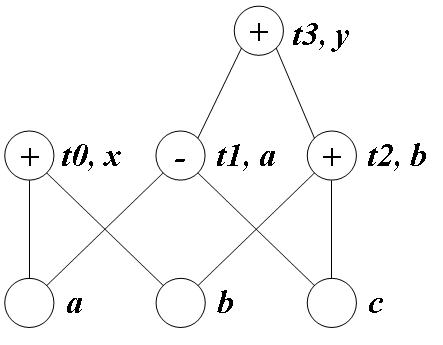
\includegraphics[width=0.7\linewidth,height=0.540\linewidth]{opt024.png}
%%\end{htmlonly}
%%\begin{latexonly}
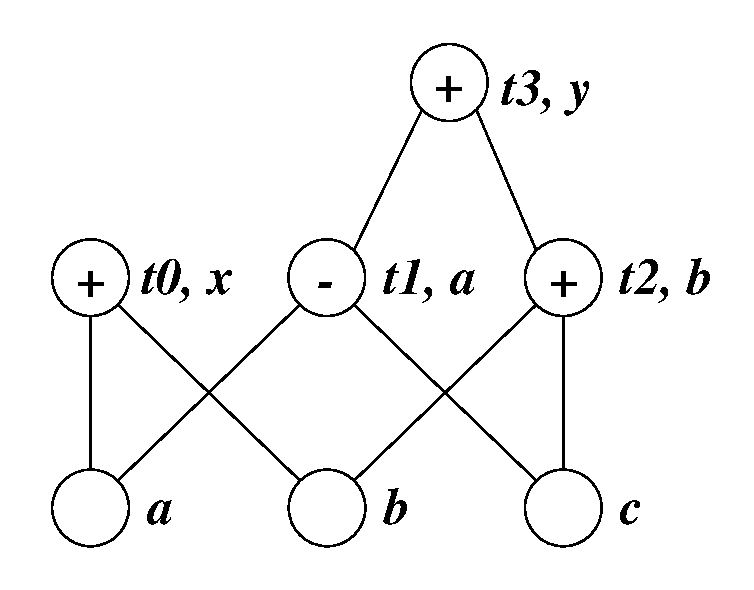
\includegraphics[width=0.7\linewidth,height=0.540\linewidth]{opt024.eps}
%%\end{latexonly}
\caption{{\em dag} of example \ref{optimize_e045}}
\label{optimize_e046}
\end{center}
\end{figure}
Function `{\tt{f}}' is consist of one basic block, and 
`{\tt{x, y}}' are alive in an exit of this basic block.
For the node whose identifier list is `{\tt{t0, x}}',
chose `{\tt{x}}' at \ref{optimize_e054} of {\bf Assignment judge algorithm}.
For the node whose identifier list is `{\tt{t1, a}}',
chose `{\tt{t1}}' at \ref{optimize_e054} of {\bf Assignment judge algorithm}.
For the node whose identifier list is `{\tt{t2, b}}',
chose `{\tt{t2}}' at \ref{optimize_e054} of {\bf Assignment judge algorithm}.
For the node whose identifier list is `{\tt{t3, y}}',
chose `{\tt{y}}' at \ref{optimize_e054} of {\bf Assignment judge algorithm}.
After appling algorithms of this section,
3 address codes become like bellow.
\begin{verbatim}
f:
   x := a + b
  t1 := a - c
  t2 := b + c
   y := t1 + t2
\end{verbatim}
\end{Example}

\begin{Example}
\label{optimize_e015}
\begin{verbatim}
int a, b, c, d; void f(void){ (a = b) + (c = d); }
\end{verbatim}
3 address codes become like bellow.
\begin{verbatim}
f:
  t0 := b
   a := t0
  t1 := d
   c := t1
  t2 := t0 + t1
\end{verbatim}
Figure \ref{optimize_e016} shows {\em dag} for these 3 address codes.
\begin{figure}[htbp]
\begin{center}
%%\begin{htmlonly}
%%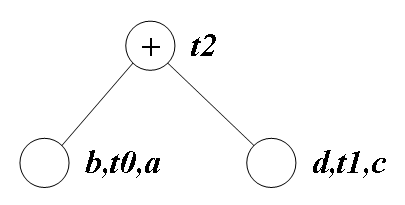
\includegraphics[width=0.7\linewidth,height=0.362\linewidth]{opt005.png}
%%\end{htmlonly}
%%\begin{latexonly}
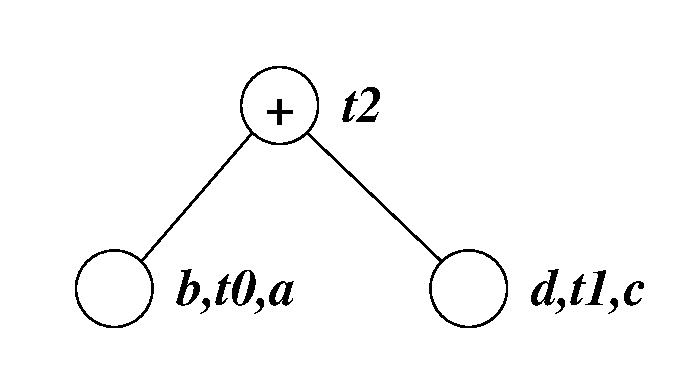
\includegraphics[width=0.7\linewidth,height=0.362\linewidth]{opt005.eps}
%%\end{latexonly}
\caption{{\em dag} of example \ref{optimize_e015}}
\label{optimize_e016}
\end{center}
\end{figure}
Function `{\tt{f}}' is consist of one basic block, and 
`{\tt{a, b, c, d}}' are alive in an exit of this basic block.
For the node whose identifier list is `{\tt{b, t0, a}}',
chose `{\tt{b}}' at \ref{optimize_e055} of {\bf Assignment judge
 algorithm}. For `{\tt{t0}}', assignment is not generated.
But for `{\tt{a}}', generate {\tt{a := b}}.
Simillary, for the node whose identifier list is `{\tt{d, t1, c}}',
chose `{\tt{d}}' at \ref{optimize_e055} of {\bf Assignment judge
 algorithm}. For `{\tt{t1}}', assignment is not generated.
But for `{\tt{d}}', generate {\tt{c := d}}.
For the node whose identifier list is `{\tt{t2}}',
3 address code {\tt{t2 := a + c}} is not generated
at \ref{optimize_e056} of {\bf Code generation algorithm from {\em dag}}
because `{\tt{t2}}' is not alive in an exit of this basic block.
After appling algorithms of this section,
3 address codes become like bellow.
\begin{verbatim}
f:
  a := b
  c := d
\end{verbatim}
\end{Example}

\begin{Example}
\begin{verbatim}
int g(void); void f(void){ g(); }
\end{verbatim}
3 address codes become like bellow.
\begin{verbatim}
f:
  t0 := call g
\end{verbatim}
Function `{\tt{f}}' is consist of one basic block.
Because `{\tt{t0}}' is not alive in an exit of this basic block,
{\tt{t0 := call g}} is converted to {\tt{call g}} at
\ref{optimize_e057} of {\bf Code generation algorithm from {\em dag}}.
\end{Example}

\begin{Example}
\label{optimize_e017}
\begin{verbatim}

int g(int);
void f(void){ int n = 2; int* p = &n; *p = 1; g(*p); }
\end{verbatim}
3 address codes become like bellow.
\begin{verbatim}
f:
   n := 2
  t0 := &n
   p := t0
  t1 := p
 *t1 := 1
  t2 := 1
  t3 := p
  t4 := *t3
  param t4
  t5 := call g
\end{verbatim}
Figure \ref{optimize_e018} shows {\em dag} at the point that
{\tt{*t1 := 1}} is processed.
\begin{figure}[htbp]
\begin{center}
%%\begin{htmlonly}
%%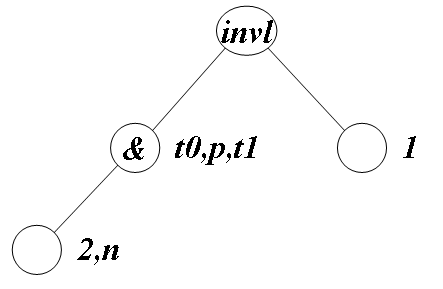
\includegraphics[width=0.8\linewidth,height=0.525\linewidth]{opt007.png}
%%\end{htmlonly}
%%\begin{latexonly}
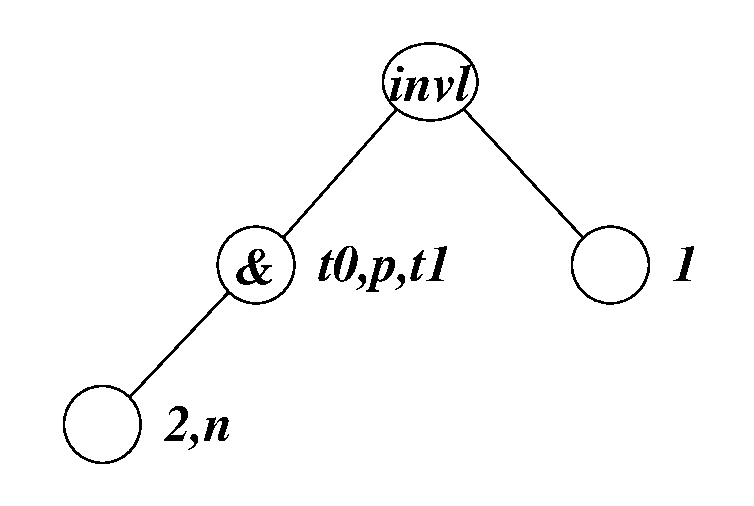
\includegraphics[width=0.8\linewidth,height=0.525\linewidth]{opt007.eps}
%%\end{latexonly}
\caption{{\em dag} of example \ref{optimize_e017}}
\label{optimize_e018}
\end{center}
\end{figure}
Function `{\tt{f}}' is consist of one basic block, and 
`{\tt{g, 1, 2}}' are alive in an exit of this basic block.
For the node whose identifier list is `{\tt{2, n}}',
chose `{\tt{2}}' at \ref{optimize_e055} of {\bf Assignment judge algorithm}.
`{\tt{n}}' is not alive in an exit of this basic block, but
the condition \ref{optimize_e052} of {\bf Assignment judge algorithm}
holds true, so generate {\tt{n := 2}} and return {\tt{n}} from
{\bf Assignment judge algorithm}.
For the node whose identifier list is `{\tt{t0, p, t1}}',
chose `{\tt{p}}' at \ref{optimize_e054} of {\bf Assignment judge
 algorithm} because `{\tt{p}}' is used later.
 `{\tt{t1}}' is not alive in an exit of this basic block,
assignment is not generated.
After appling algorithms of this section,
this {\em dag} is converted to like bellow.
\begin{verbatim}
  n := 2
  p := &n
 *p := 1
\end{verbatim}
The best codes for `{\tt{f}}' are
\begin{verbatim}
f:
  param 1
  call g
\end{verbatim}
But in this section, no more discussion for the best codes.
\end{Example}

\begin{Example}
\label{optimize_e023}
\begin{verbatim}
int f(void){ int n = 2; int* p = &n; *p = 1; return *p; }
\end{verbatim}
3 address codes become like bellow.
\begin{verbatim}
f:
   n := 2
  t0 := &n
   p := t0
  t1 := p
 *t1 := 1
  t2 := 1
  t3 := p
  t4 := *t3
  return t4
\end{verbatim}
Figure \ref{optimize_e024} shows {\em dag} at the point
that {\tt{*t1 := 1}} is processed.
\begin{figure}[htbp]
\begin{center}
%%\begin{htmlonly}
%%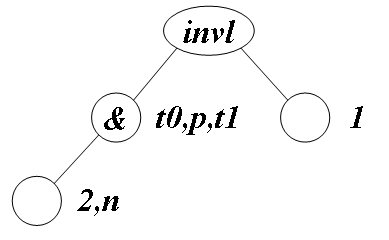
\includegraphics[width=0.7\linewidth,height=0.423\linewidth]{opt010.png}
%%\end{htmlonly}
%%\begin{latexonly}
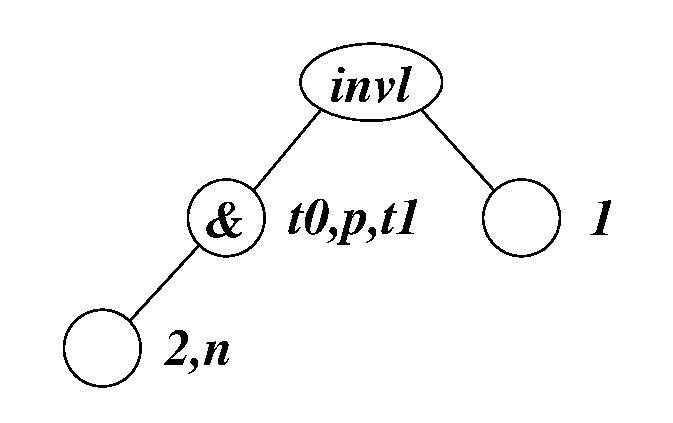
\includegraphics[width=0.7\linewidth,height=0.423\linewidth]{opt010.eps}
%%\end{latexonly}
\caption{{\em dag} of example \ref{optimize_e023}}
\label{optimize_e024}
\end{center}
\end{figure}
Function `{\tt{f}}' is consist of one basic block, and 
`{\tt{1, 2}}' is alive in an exit of this basic block.
For the node whose identifier list is `{\tt{2, n}}',
chose `{\tt{2}}' at \ref{optimize_e055} of {\bf Assignment judge algorithm}.
`{\tt{n}}' is not alive in an exit of this basic block,
but {\tt{n := 2}} is generated becase of \ref{optimize_e052}
of {\bf Assignment judge algorithm}. And return `{\tt{n}}'
form {\bf Assignment judge algorithm}.
For the node whose identifier list is `{\tt{t0, p, t1}}',
chose `{\tt{p}}' at \ref{optimize_e054} of {\bf Assignment judge
 algorithm} because `{\tt{p}}' is used later.
`{\tt{t1}}' is not alive in an exit of this basic block,
so assignment is not genearted.
After appling algorithms of this section,
3 address codes become like bellow.
\begin{verbatim}
  n := 2
  p := &n
 *p := 1
\end{verbatim}
The best codes for `{\tt{f}}' are
\begin{verbatim}
f:
  return 1
\end{verbatim}
But in this section, no more discussion for the best codes.
\end{Example}

\begin{Example}
\label{optimize_e019}
\begin{verbatim}
int g(int); void f(void){ int n = 2; int* p = &n; g(*p); }
\end{verbatim}
3 address codes become like bellow.
\begin{verbatim}
f:
   n := 2
  t0 := &n
   p := t0
  t1 := p
  t2 := *t1
  param t2
  t3 := call g
\end{verbatim}
Figure \ref{optimize_e020} shows {\em dag} for these 3 address codes.
\begin{figure}[htbp]
\begin{center}
%%\begin{htmlonly}
%%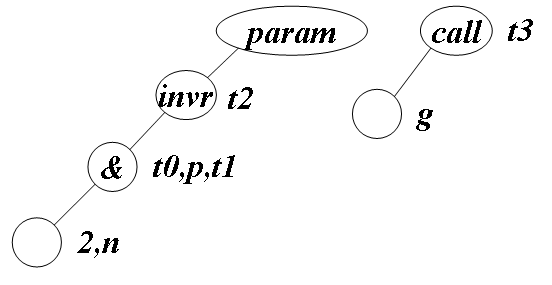
\includegraphics[width=1.0\linewidth,height=0.507\linewidth]{opt008.png}
%%\end{htmlonly}
%%\begin{latexonly}
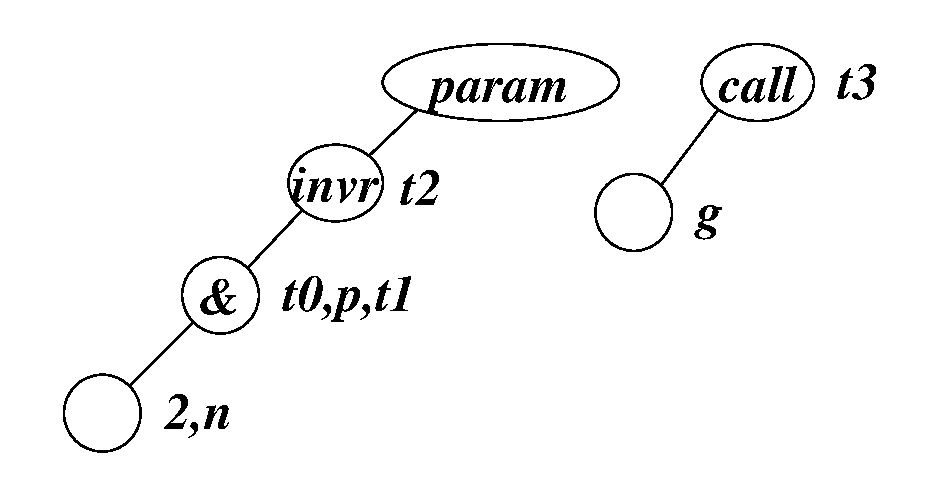
\includegraphics[width=1.0\linewidth,height=0.507\linewidth]{opt008.eps}
%%\end{latexonly}
\caption{{\em dag} of example \ref{optimize_e019}}
\label{optimize_e020}
\end{center}
\end{figure}
Function `{\tt{f}}' is consist of one basic block, and 
`{\tt{g, 2}}' are alive in an exit of this basic block.
For the node whose identifier list is `{\tt{t2, n}}',
chose `{\tt{2}}' at \ref{optimize_e055} of {\bf Assignment judge algorithm}.
`{\tt{n}}' is not alive in an exit of this block,
but {\tt{n := 2}} is generated becase of \ref{optimize_e052}
of {\bf Assignment judge algorithm}. And return `{\tt{n}}'
For the node whose identifier list is `{\tt{t0, p, t1}}',
chose `{\tt{t0}}' at \ref{optimize_e054} of {\bf Assignment judge algorithm}.
After appling algorithms of this section,
3 address codes become like bellow.
\begin{verbatim}
f:
   n := 2
  t0 := &n
  t2 := *t0
  param t2
  call g
\end{verbatim}
The best codes for `{\tt{f}}' are
\begin{verbatim}
f:
  param 2
  call g
\end{verbatim}
But in this section, no more discussion for the best codes.
\end{Example}

\begin{Example}
\label{optimize_e021}
\begin{verbatim}
void g(int, int); void f(int x){ g(x+1,x+2); }
\end{verbatim}
3 address codes become like bellow.
\begin{verbatim}
f:
  t0 := x + 1
  t1 := x + 2
  param t0
  param t1
  call g
\end{verbatim}
Figure \ref{optimize_e022} shows {\em dag} for these 3 address codes.
\begin{figure}[htbp]
\begin{center}
%%\begin{htmlonly}
%%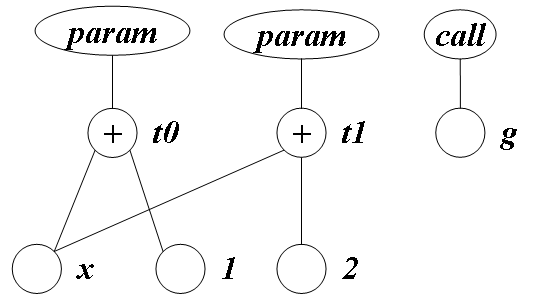
\includegraphics[width=0.8\linewidth,height=0.470\linewidth]{opt009.png}
%%\end{htmlonly}
%%\begin{latexonly}
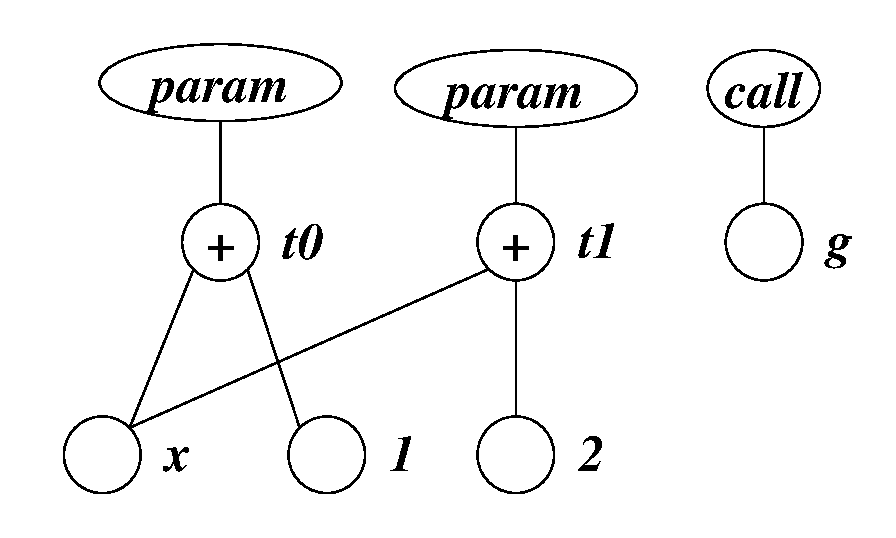
\includegraphics[width=0.8\linewidth,height=0.470\linewidth]{opt009.eps}
%%\end{latexonly}
\caption{{\em dag} of example \ref{optimize_e021}}
\label{optimize_e022}
\end{center}
\end{figure}
Similary so far, applying {\bf Code generation algorithm from {\em
 dag}}, and get the same 3 address codes.
As we described at \ref{_3ac_e000}, frontend must 
generate {\tt{param}} or {\tt{param}}s continually
which is or are referenced by {\tt{call}}, just before generating
{\tt{call}}, and the constraint is kept after optimization.
\end{Example}

\begin{Example}
\label{optimize_e025}
\begin{verbatim}
void f(int* p){ --*p; }
\end{verbatim}
3 address codes become like bellow.
\begin{verbatim}
f:
  t0 := p
  t1 := *t0
  t1 := t1 - 1
 *t0 := t1
\end{verbatim}
Figure \ref{optimize_e026} shows {\em dag} for these 3 address codes.
\begin{figure}[htbp]
\begin{center}
%%\begin{htmlonly}
%%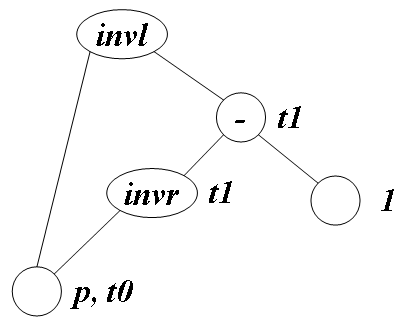
\includegraphics[width=0.7\linewidth,height=0.552\linewidth]{opt011.png}
%%\end{htmlonly}
%%\begin{latexonly}
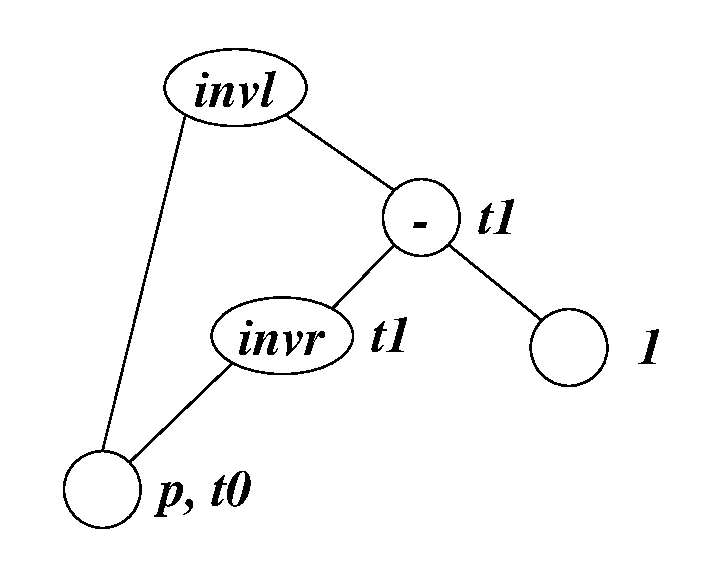
\includegraphics[width=0.7\linewidth,height=0.552\linewidth]{opt011.eps}
%%\end{latexonly}
\caption{{\em dag} of example \ref{optimize_e025}}
\label{optimize_e026}
\end{center}
\end{figure}
Function `{\tt{f}}' is consist of one basic block, and 
`{\tt{1}}' is alive in an exit of this basic block.
For the node whose identifier list is `{\tt{p, t0}}',
chose `{\tt{p}}' at \ref{optimize_e055} of {\bf Assignment judge
 algorithm}.
`{\tt{t0}}' is not alive in an exit of this basic block, so
assignment is not generated.
After appling algorithms of this section,
3 address codes become like bellow.
\begin{verbatim}
f:
  t1 := *p
  t1 := t1 - 1
  *p := t1
\end{verbatim}
\end{Example}

\begin{Example}
\label{optimize_e027}
\begin{verbatim}
void g(double, int, int);
void f(double d){ int a = (int)d; int b = a; g(d,a,b); }
\end{verbatim}
3 address codes become like bellow.
\begin{verbatim}
f:
  t0 := (int)d
   a := t0
  t1 := a
   b := t1
  t2 := d
  t3 := a
  t4 := b
  param t2
  param t3
  param t4
  call g
\end{verbatim}
Figure \ref{optimize_e028} shows {\em dag} for these 3 address codes.
\begin{figure}[htbp]
\begin{center}
%%\begin{htmlonly}
%%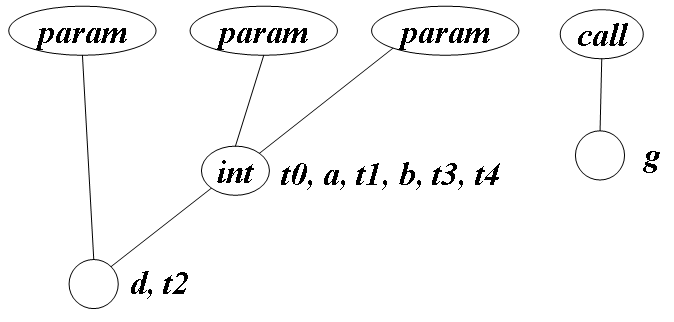
\includegraphics[width=1.0\linewidth,height=0.483\linewidth]{opt012.png}
%%\end{htmlonly}
%%\begin{latexonly}
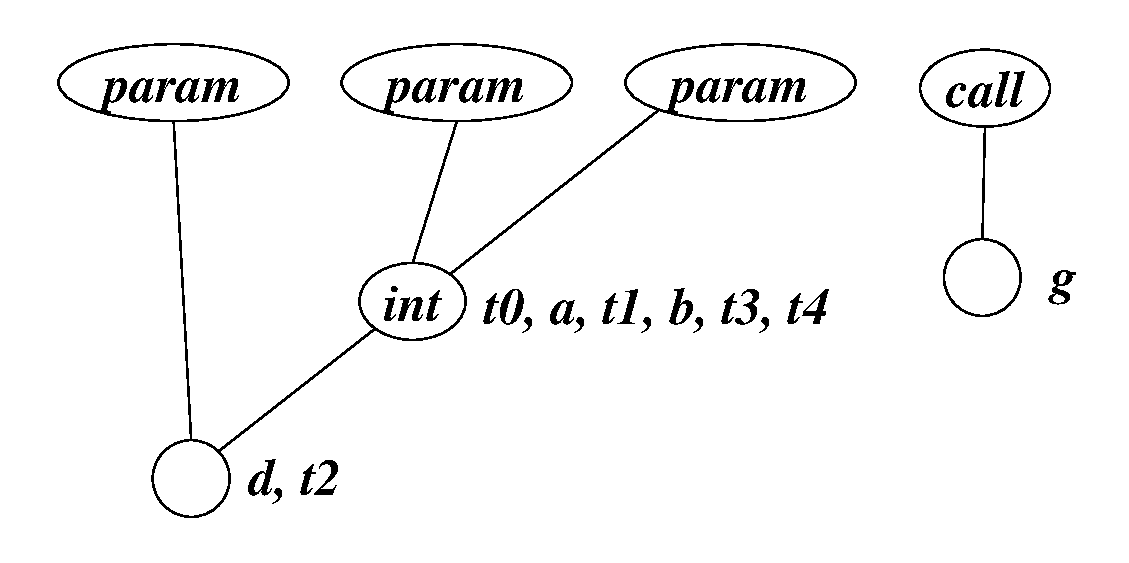
\includegraphics[width=1.0\linewidth,height=0.483\linewidth]{opt012.eps}
%%\end{latexonly}
\caption{{\em dag} of example \ref{optimize_e027}}
\label{optimize_e028}
\end{center}
\end{figure}
Function `{\tt{f}}' is consist of one basic block, and 
`{\tt{g}}' is alive in an exit of this basic block.
For the node whose identifier list is `{\tt{d, t2}}',
chose `{\tt{d}}' at \ref{optimize_e055} of {\bf Assignment judge
 algorithm}.
`{\tt{t2}}' is not alive in an exit of this basic block, so
assignment is not generated.
For the node whose identifier list is `{\tt{t0, a, t1, b, t3, t4}}',
chose `{\tt{t0}}' at \ref{optimize_e054} of {\bf Assignment judge
 algorithm}.
`{\tt{a, t1, b, t3, t4}}' are not alive in an exit of this basic block, so
assignments are not generated.
After appling algorithms of this section,
3 address codes become like bellow.
\begin{verbatim}
f:
  t0 := (int)d
  param d
  param t0
  param t0
  call g
\end{verbatim}
\end{Example}

\begin{Example}
\label{optimize_e029}
\begin{verbatim}
int n; int g(int); void f(void){ n = 2; n = g(3); ++n; }
\end{verbatim}
3 address codes become like bellow.
\begin{verbatim}
f:
   n := 2
  t0 := 2
  param 3
  t1 := call g
   n := t1
   n := n + 1
  t2 := n
\end{verbatim}
Figure \ref{optimize_e030} shows {\em dag} for these 3 address codes.
Here, the upper of figure \ref{optimize_e030} is {\em dag}
at the point that {\tt{t1 := call g}} is processed.
\begin{figure}[htbp]
\begin{center}
%%\begin{htmlonly}
%%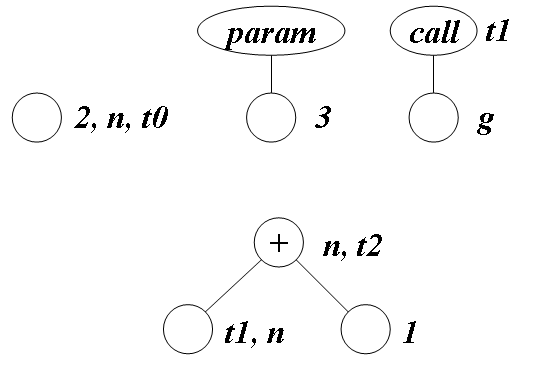
\includegraphics[width=0.8\linewidth,height=0.571\linewidth]{opt013.png}
%%\end{htmlonly}
%%\begin{latexonly}
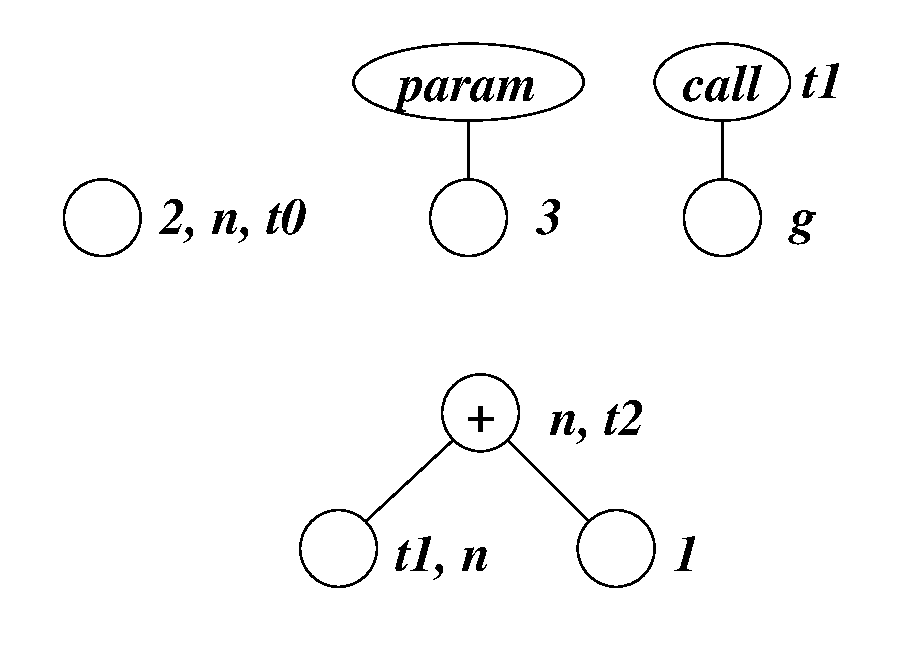
\includegraphics[width=0.8\linewidth,height=0.571\linewidth]{opt013.eps}
%%\end{latexonly}
\caption{{\em dag} of example \ref{optimize_e029}}
\label{optimize_e030}
\end{center}
\end{figure}
Function `{\tt{f}}' is consist of one basic block.
`{\tt{g, n, 1, 2, 3}}' are alive in an exit of the this basic block.

For the node whose identifier list is `{\tt{2, n, t0}}',
chose `{\tt{2}}' at \ref{optimize_e054} of {\bf Assignment judge
 algorithm}.
`{\tt{n}}' is alive in an exit of this basic block, so
{\tt{n := 2}} is generated. But
`{\tt{t0}}' is not alive in an exit of this basic block, so
assignment is not generated.
The upper {\em dag} of the figure \ref{optimize_e030} 
is converted to like bellow.
\begin{verbatim}
   n := 2
  pamar 3
  t1 := call g
\end{verbatim}
For the node whose identifier list is `{\tt{t1, n}}',
chose `{\tt{t1}}' at \ref{optimize_e054} of {\bf Assignment judge
 algorithm}.
`{\tt{n}}' is alive in an exit of this basic block, but
assignment is not generated because {\tt{node[n]}} is
not equalt to this node.
For the node whose identifier list is `{\tt{n, t2}}',
`{\tt{t2}}' is not alive in an exit of this basic block, 
so assignment is not generated.
The lower {\em dag} of the figure \ref{optimize_e030} 
is converted to like bellow.
\begin{verbatim}
   n := t1 + 1
\end{verbatim}
Finally, 3 address codes becomes like bellow.
\begin{verbatim}
f:
   n := 2
  pamar 3
  t1 := call g
   n := t1 + 1
\end{verbatim}
\end{Example}

\begin{Example}
\label{optimize_e031}
\begin{verbatim}
void g(char*); void f(void){ char s[] = "abc"; g(s); }
\end{verbatim}
3 address codes become like bellow.
\begin{verbatim}
f:
    t0 := &"abc"
  s[0] := 'a'
  s[1] := 'b'
  s[2] := 'c'
  s[3] := '\0'
    t1 := &s
    t2 := t1
    param t2
    call g
\end{verbatim}
Figure \ref{optimize_e032} shows {\em dag} for these 3 address codes.
\begin{figure}[htbp]
\begin{center}
%%\begin{htmlonly}
%%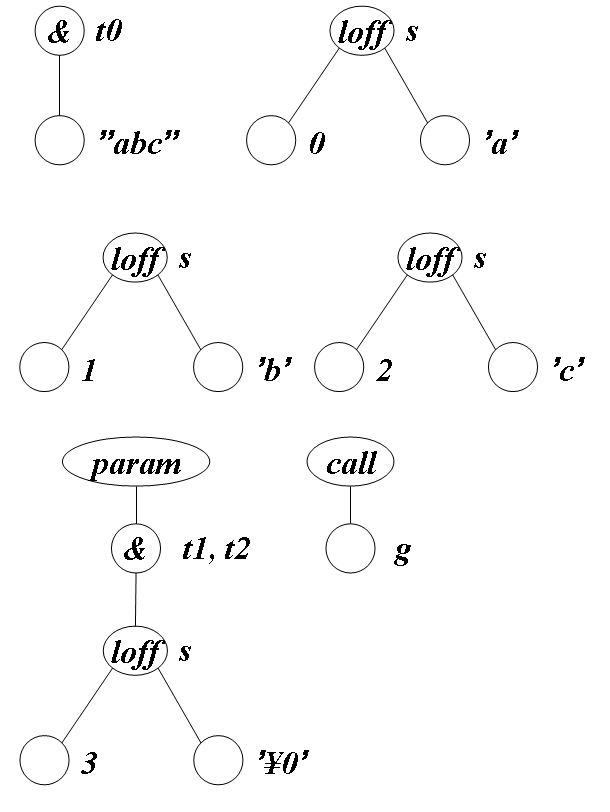
\includegraphics[width=0.859\linewidth,height=1.0\linewidth]{opt016.png}
%%\end{htmlonly}
%%\begin{latexonly}
%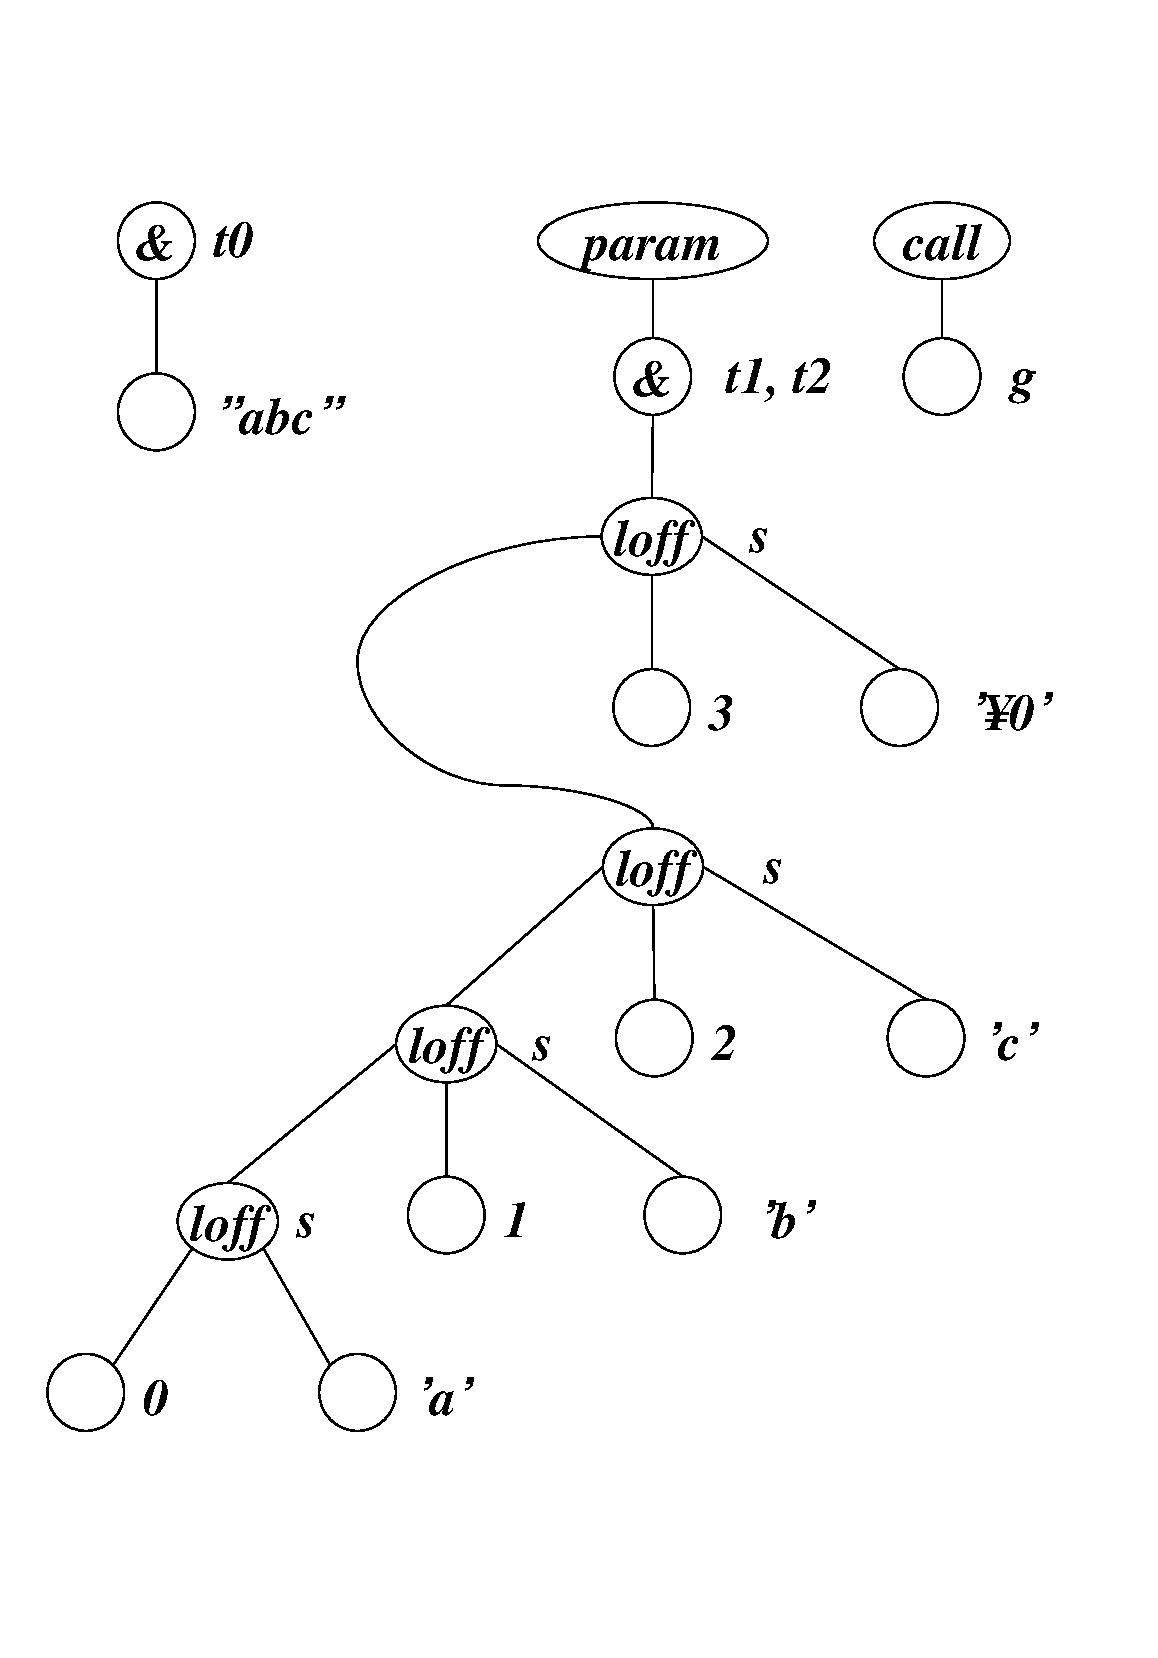
\includegraphics[width=0.859\linewidth,height=1.0\linewidth]{opt016.eps}
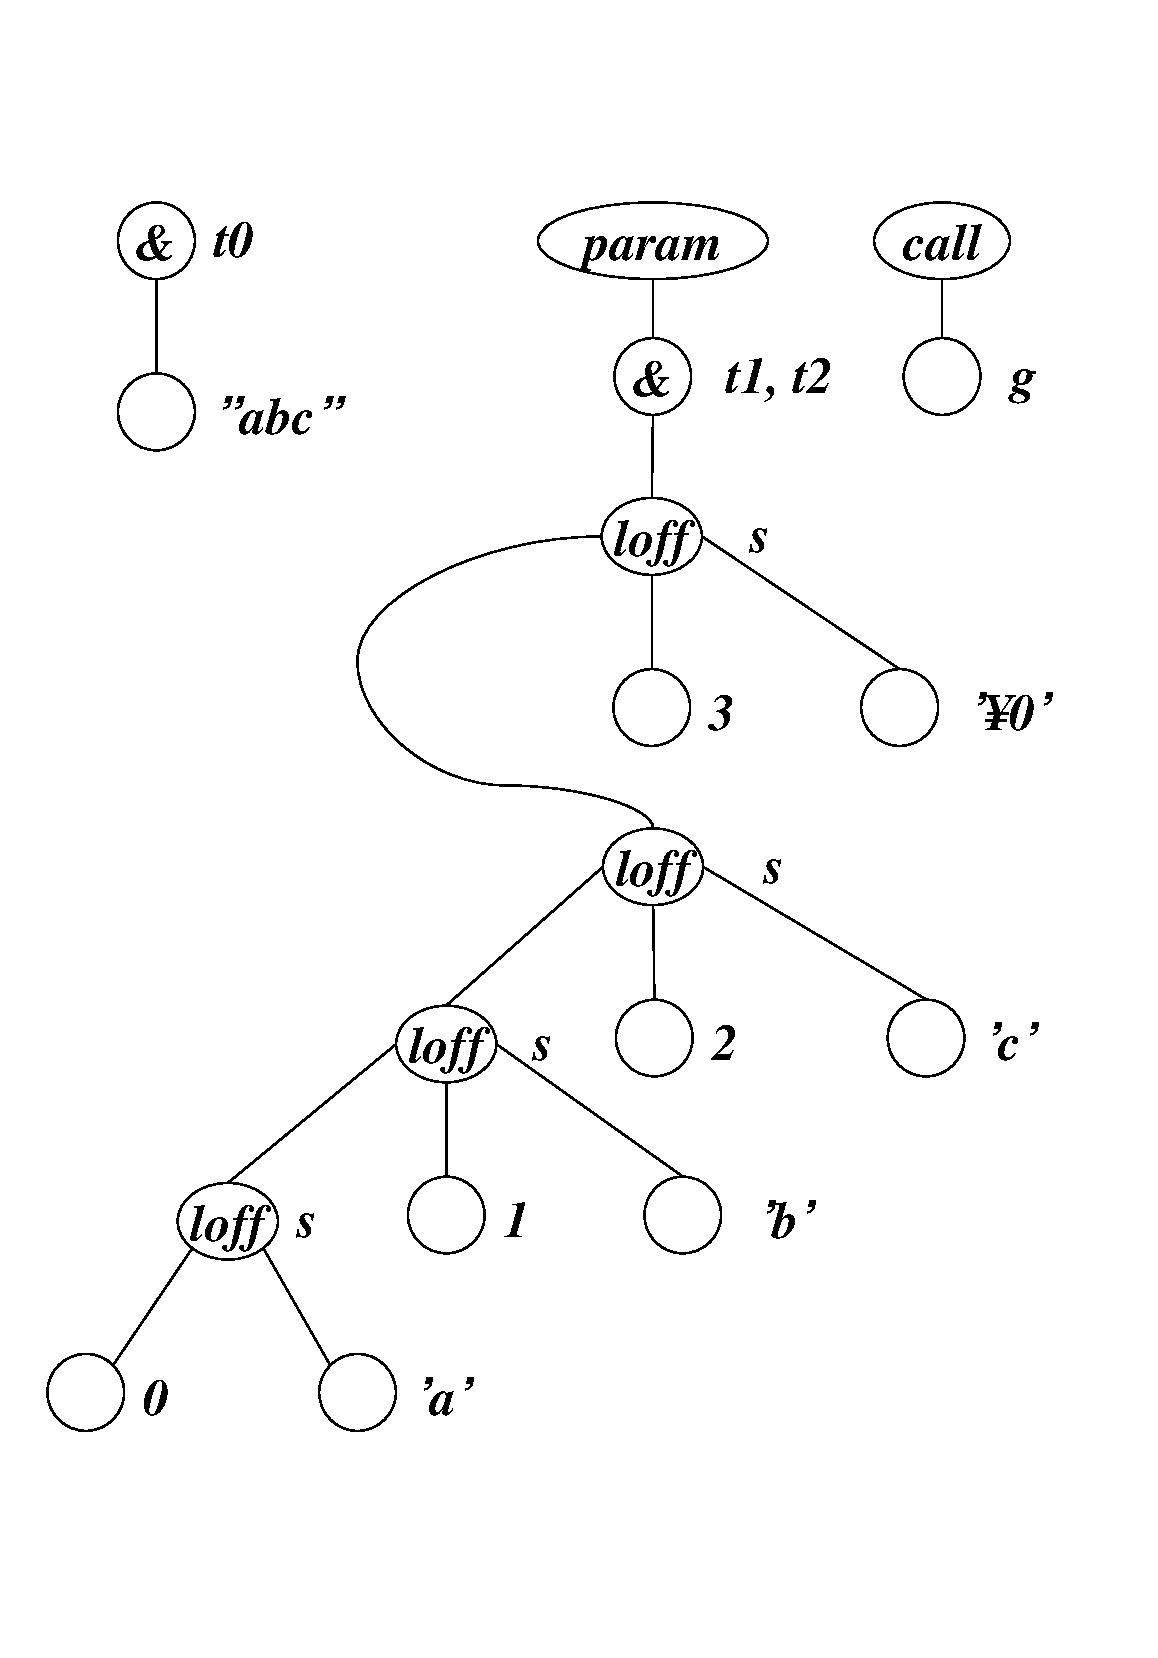
\includegraphics[width=1.0\linewidth,height=1.2\linewidth]{opt016.eps}
%%\end{latexonly}
\caption{{\em dag} of example \ref{optimize_e031}}
\label{optimize_e032}
\end{center}
\end{figure}
Function `{\tt{f}}' is consist of one basic block, and 
`{\tt{g, "abc", 0, 1, 2, 3, 'a', 'b', 'c', '\verb|\|0'}}'
are alive in an exit of this basic block.
Here, think about nodes whose label is {\tt{loff}} except for 1st one.
They have 3rd child.
`{\tt{s}}' is not alive in an exit of this basic block,
this 3 address code may be omitted if they don't have 3rd child.
But function `{\tt{g}}' call argument is address of `{\tt{s}}'
and we can easyly know that they cannot be omitted.
At \ref{optimize_e064} of {\bf Code generation algorithm from {\em dag}},
{\tt{x[y] := z}} is treated specially for such a reason.
After appling algorithms of this section,
3 address codes become like bellow.
\begin{verbatim}
f:
  s[0] := 'a'
  s[1] := 'b'
  s[2] := 'c'
  s[3] := '\0'
  t1 := &s
  param t1
  call g
\end{verbatim}
\end{Example}

\begin{Example}
\label{optimize_e033}
\begin{verbatim}
void g(int); void f(void){ int n = 1; n = 2; g(n); }
\end{verbatim}
3 address codes become like bellow.
\begin{verbatim}
f:
   n := 1
   n := 2
  t0 := 2
  t1 := n
  param t1
  call g
\end{verbatim}
Figure \ref{optimize_e034} shows {\em dag} for these 3 address codes.
\begin{figure}[htbp]
\begin{center}
%%\begin{htmlonly}
%%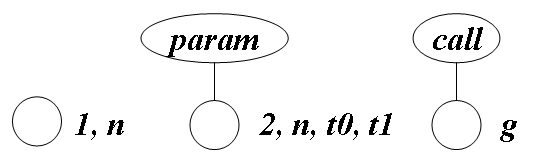
\includegraphics[width=0.8\linewidth,height=0.247\linewidth]{opt018.png}
%%\end{htmlonly}
%%\begin{latexonly}
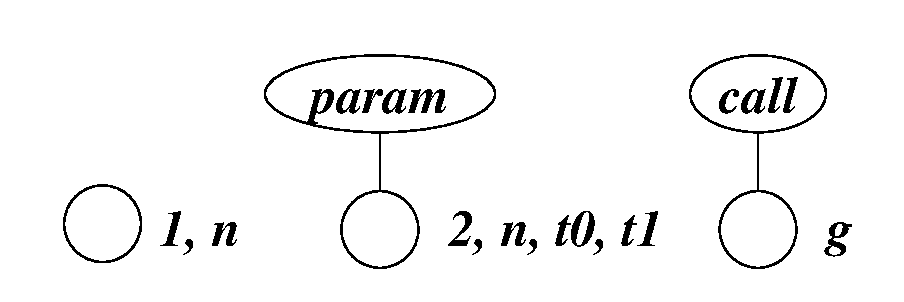
\includegraphics[width=0.8\linewidth,height=0.247\linewidth]{opt018.eps}
%%\end{latexonly}
\caption{{\em dag} of example \ref{optimize_e033}}
\label{optimize_e034}
\end{center}
\end{figure}
After appling algorithms of this section,
3 address codes become like bellow.
\begin{verbatim}
f:
  param 2
  call g
\end{verbatim}
\end{Example}

\begin{Example}
\label{optimize_e037}
\begin{verbatim}
void g(int*, int*); void f(void){ int i[2]; g(&i[0],&i[1]); }
\end{verbatim}
3 address codes become like bellow.
\begin{verbatim}
f:
  t0 := &i
  t1 := &i
  t1 := t1 + 4
  param t0
  param t1
  call g
\end{verbatim}
Figure \ref{optimize_e038} shows {\em dag} for these 3 address codes.
\begin{figure}[htbp]
\begin{center}
%%\begin{htmlonly}
%%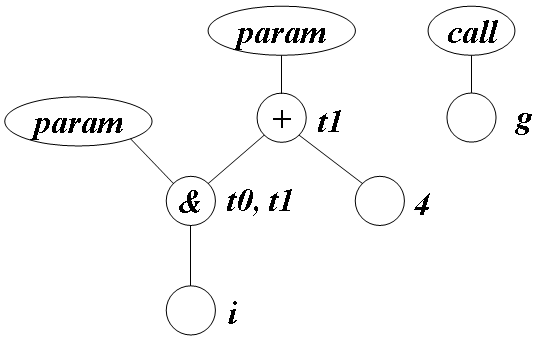
\includegraphics[width=1.0\linewidth,height=0.623\linewidth]{opt020.png}
%%\end{htmlonly}
%%\begin{latexonly}
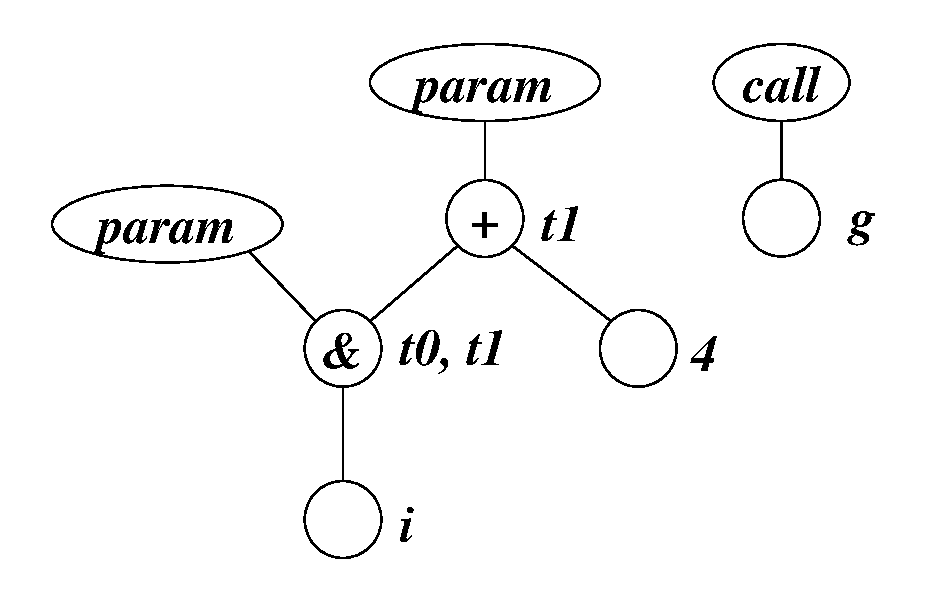
\includegraphics[width=1.0\linewidth,height=0.623\linewidth]{opt020.eps}
%%\end{latexonly}
\caption{{\em dag} of example \ref{optimize_e037}}
\label{optimize_e038}
\end{center}
\end{figure}
After appling algorithms of this section,
3 address codes become like bellow.
\begin{verbatim}
f:
  t0 := &i
  t1 := t0 + 4
  param t0
  param t1
  call g
\end{verbatim}
\end{Example}

\begin{Example}
\label{optimize_e065}
\begin{verbatim}
int n; void g(int); void f(void){ g(n++); }
\end{verbatim}
3 address codes become like bellow.
\begin{verbatim}
f:
  t0 := n
   n := n + 1
  param t0
  call g
\end{verbatim}
Figure \ref{optimize_e066} shows {\em dag} for these 3 address codes.
\begin{figure}[htbp]
\begin{center}
%%\begin{htmlonly}
%%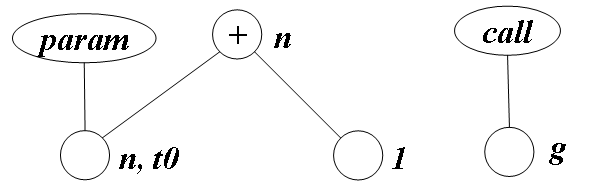
\includegraphics[width=1.0\linewidth,height=0.328\linewidth]{opt027.png}
%%\end{htmlonly}
%%\begin{latexonly}
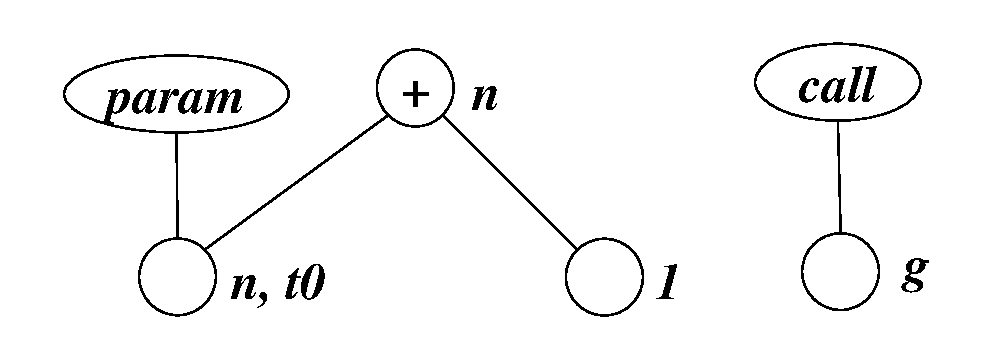
\includegraphics[width=1.0\linewidth,height=0.328\linewidth]{opt027.eps}
%%\end{latexonly}
\caption{{\em dag} of example \ref{optimize_e065}}
\label{optimize_e066}
\end{center}
\end{figure}
Applying {\bf Assignment judge
 algorithm} to the node whose identifier list is `{\tt{n, t0}}',
this is in the case
of {\bf Assignment judge algorithm (Special case 1)}
because {\tt{node[n]}} is not equal to this node and
{\tt{node[t0]}} is equal to this node.
As a result, {\tt{t0 := n}} is generated.
Finally, 3 address codes become like bellow.
\begin{verbatim}
f:
  t0 := n
   n := t0 + 1
  param t0
  call g
\end{verbatim}
\end{Example}

\begin{Example}
\label{optimize_e068}
\begin{verbatim}

struct S { unsigned int a : 1; unsigned int b : 2; };
extern struct S s; unsigned int f(void){ return s.a + s.b; }
\end{verbatim}
3 address codes become like bellow.
\begin{verbatim}
f:
  t0 := s[0]
  t1 := t0 & 1
  t2 := s[0]
  t3 := t2 >> 1
  t4 := t3 & 3
  t5 := t1 + t4
  return t5
\end{verbatim}
Figure \ref{optimize_e069} shows {\em dag} for these 3 address codes.
\begin{figure}[htbp]
\begin{center}
%%\begin{htmlonly}
%%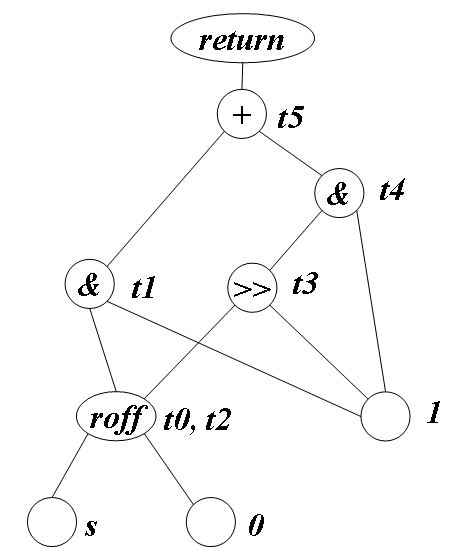
\includegraphics[width=0.826\linewidth,height=1.0\linewidth]{opt028.png}
%%\end{htmlonly}
%%\begin{latexonly}
\includegraphics[width=0.826\linewidth,height=1.0\linewidth]{opt028.eps}
%%\end{latexonly}
\caption{{\em dag} of example \ref{optimize_e068}}
\label{optimize_e069}
\end{center}
\end{figure}
Similary so far, frontend can detect common expression {\tt{s[0]}}
by applying {\bf Code generation algorithm from {\em dag}}.
After appling algorithms of this section,
3 address codes become like bellow.
\begin{verbatim}
f:
  t0 := s[0]
  t1 := t0 & 1
  t3 := t0 >> 1
  t4 := t3 & 3
  t5 := t1 + t4
  return t5
\end{verbatim}
\end{Example}

\begin{Example}
\label{optimize_e070}
\begin{verbatim}
int f(void){ static int s; return s++; }
\end{verbatim}
3 address codes become like bellow.
\begin{verbatim}
f:
  t0 := s
   s := s + 1
  return t0
\end{verbatim}
Figure \ref{optimize_e071} shows {\em dag} for these 3 address codes.
\begin{figure}[htbp]
\begin{center}
%%\begin{htmlonly}
%%\includegraphics[width=0.8\linewidth,height=0.347\linewidth]{opt029.png}
%%\end{htmlonly}
%%\begin{latexonly}
\includegraphics[width=0.8\linewidth,height=0.347\linewidth]{opt029.eps}
%%\end{latexonly}
\caption{{\em dag} of example \ref{optimize_e070}}
\label{optimize_e071}
\end{center}
\end{figure}
The node whose identifier list is `{\tt{s, t0}}'
is in case of {\bf Assignment judge algorithm (Special case 1) },
so, {\tt{t0 := s}} is generated and the result of this node
is `{\tt{t0}}' not `{\tt{s}}'.
After appling algorithms of this section,
3 address codes become like bellow.
\begin{verbatim}
f:
  t0 := s
   s := t0 + 1
  return t0
\end{verbatim}
\end{Example}

\begin{Example}
\label{optimize_e073}
\begin{verbatim}

struct S { int m; int n; }; void g(struct S);
void f(void){ struct S x, y = { 1, 2 }; x = y; g(x); }
\end{verbatim}
3 address codes become like bellow.
\begin{verbatim}
f:
  y[0] := 1
  y[4] := 2
    t0 := y
     x := t0
    t1 := x
  param t1
  call g
\end{verbatim}
Figure \ref{optimize_e074} shows {\em dag} for these 3 address codes.
\begin{figure}[htbp]
\begin{center}
%%\begin{htmlonly}
%%\includegraphics[width=1.0\linewidth,height=0.439\linewidth]{opt030.png}
%%\end{htmlonly}
%%\begin{latexonly}
%\includegraphics[width=1.0\linewidth,height=0.439\linewidth]{opt030.eps}
\includegraphics[width=1.2\linewidth,height=1.0\linewidth]{opt030.eps}
%%\end{latexonly}
\caption{{\em dag} of example \ref{optimize_e073}}
\label{optimize_e074}
\end{center}
\end{figure}
Function `{\tt{f}}' is consist of one basic block, and 
`{\tt{g, 0, 1, 2, 4}}' are alive in an exit of this basic block.
Because `{\tt{y}}' is not alive in an exit of this basic block,
it's necessary to have parent of the node whose label is {\tt{y[0] := 1}}
for generating code.
3 address codes become like bellow.
\begin{verbatim}
f:
  y[0] := 1
  y[4] := 2
    t0 := y  # Canbe erased.
     x := y  # But this algorithm cannot erase
    t1 := y  # at present state.
  param y
  call g
\end{verbatim}
\end{Example}

\begin{Example}
\label{optimize_e077}
\begin{verbatim}

void g(int, int*, int*);
void f(void)
{ int a = 0; int b = 1; int c = 2; g(a,&b,&c); ++a; g(a,&b,&c); }
\end{verbatim}
3 address codes become like bellow.
\begin{verbatim}
f:
  a := 0
  b := 1
  c := 2
  t0 := &b
  t1 := &c
  t2 := a
  param t2
  param t0
  param t1
  call g
  a := a + 1
  t3 := a
  t4 := &b
  t5 := &c
  t6 := a
  param t6
  param t4
  param t5
  call g
\end{verbatim}
Figure \ref{optimize_e078} shows {\em dag} for these 3 address codes.
\begin{figure}[htbp]
\begin{center}
%%\begin{htmlonly}
%%\includegraphics[width=1.0\linewidth,height=0.894\linewidth]{opt032.png}
%%\end{htmlonly}
%%\begin{latexonly}
\includegraphics[width=1.0\linewidth,height=0.894\linewidth]{opt032.eps}
%%\end{latexonly}
\caption{{\em dag} of example \ref{optimize_e077}}
\label{optimize_e078}
\end{center}
\end{figure}
Similary so far,
after appling algorithms of this section,
3 address codes become like bellow.
\begin{verbatim}
f:
  a := 0
  b := 1
  c := 2
  t0 := &b
  t1 := &c
  param 0
  param t0
  param t1
  call g
  a := a + 1
  t4 := &b
  t5 := &c
  param a
  param t4
  param t5
  call g
\end{verbatim}
\end{Example}

\begin{Example}
\label{optimize_e079}
\begin{verbatim}

void g(void); struct S { int a; }; void h(struct S);
void f(struct S y){ struct S x = { 1 }; g(); x = y; h(x); }
\end{verbatim}
3 address codes become like bellow.
\begin{verbatim}
f:
  x[0] := 1
  call g
  t0 := y
  x := t0
  t1 := x
  param t1
  call h
\end{verbatim}
Figure \ref{optimize_e080} shows {\em dag} for these 3 address codes.
Here, the upper of figure \ref{optimize_e080} is {\em dag}
at the point that {\tt{call g}} is processed.
\begin{figure}[htbp]
\begin{center}
%%\begin{htmlonly}
%%\includegraphics[width=0.6\linewidth,height=0.6\linewidth]{opt033.png}
%%\end{htmlonly}
%%\begin{latexonly}
\includegraphics[width=0.6\linewidth,height=0.6\linewidth]{opt033.eps}
%%\end{latexonly}
\caption{{\em dag} of example \ref{optimize_e079}}
\label{optimize_e080}
\end{center}
\end{figure}
Function `{\tt{f}}' is consist of one basic block, and 
`{\tt{x}}' is not alive in exit of this basic block.
For this reason, no code is generated
for the node whose label is {\tt{x[0] :=
 1}} in the upper {\em dag} of figure \ref{optimize_e080}.
For the node whose identifier list is `{\tt{y, t0, x, t1}}',
chose `{\tt{y}}' at \ref{optimize_e055} of {\bf Assignment judge
algorithm}, and no assignment is generated for `{\tt{t0, x, t1}}'.
After appling algorithms of this section,
3 address codes become like bellow.
\begin{verbatim}
f:
  call g
  param y
  call h
\end{verbatim}
\end{Example}

\begin{Example}
\label{optimize_e081}
\begin{verbatim}

struct S { int a; }; void g(struct S);
void f(struct S y){ struct S x = { 1 }; g(x); x = y; g(x); }
\end{verbatim}
3 address codes become like bellow.
\begin{verbatim}
f:
  x[0] := 1
  t0 := x
  param t0
  call g
  t1 := y
  x := t1
  t2 := x
  param t2
  call g
\end{verbatim}
Figure \ref{optimize_e082} shows {\em dag} for these 3 address codes.
\begin{figure}[htbp]
\begin{center}
%%\begin{htmlonly}
%%\includegraphics[width=0.493\linewidth,height=0.6\linewidth]{opt034.png}
%%\end{htmlonly}
%%\begin{latexonly}
\includegraphics[width=0.493\linewidth,height=0.6\linewidth]{opt034.eps}
%%\end{latexonly}
\caption{{\em dag} of example \ref{optimize_e081}}
\label{optimize_e082}
\end{center}
\end{figure}
Function `{\tt{f}}' is consist of one basic block.
For the node whose identifier list is `{\tt{y, t1, x, t2}}',
chose `{\tt{y}}' and no assignment is generated for
{\tt{t1, x, t2}} becase they are not alive in an exit
of this basic block.
After appling algorithms of this section,
3 address codes become like bellow.
\begin{verbatim}
f:
  x[0] := 1
  param x
  call g
  param y
  call g
\end{verbatim}
\end{Example}

\begin{Example}
\label{optimize_e083}
\begin{verbatim}
void g(int); int x[3][5]; void f(void){ g(x[2][3]); }
\end{verbatim}
3 address codes become like bellow.
\begin{verbatim}
f:
  t0 := &x
  t1 := t0 + 40
  t2 := x[52]
  param t2
  call g
\end{verbatim}
Figure \ref{optimize_e084} shows {\em dag} for these 3 address codes.
\begin{figure}[htbp]
\begin{center}
%%\begin{htmlonly}
%%\includegraphics[width=1.0\linewidth,height=0.509\linewidth]{opt035.png}
%%\end{htmlonly}
%%\begin{latexonly}
\includegraphics[width=1.0\linewidth,height=0.509\linewidth]{opt035.eps}
%%\end{latexonly}
\caption{{\em dag} of example \ref{optimize_e083}}
\label{optimize_e084}
\end{center}
\end{figure}
Function `{\tt{f}}' is consist of one basic block,
and `{\tt{t0, t1, t2}}' is not alive in an exit of this basic block.
Similary so far, 
after appling algorithms of this section,
3 address codes become like bellow.
\begin{verbatim}
f:
  t0 := &x
  t2 := x[52]
  param t2
  call g
\end{verbatim}
Here, {\tt{t0 := \&x}} can be ommited if 
applying {\bf Creation {\em dag} of basic block algorithm} an
{\bf Code generation algorithm from {\em dag}} again.
\end{Example}

\begin{Example}
\label{optimize_e075}
\begin{verbatim}

extern int a[];
void f(int i, int j){ int x = a[i]; a[i] = a[j]; a[j] =	x; }
\end{verbatim}
3 address codes become like bellow.
\begin{verbatim}
f:
    t0 := i << 2
    t1 := a[t0]
     x := t1
    t2 := i << 2
    t3 := j << 2
    t4 := a[t3]
 a[t2] := t4
    t5 := j << 2
    t6 := x
 a[t5] := t6
\end{verbatim}
Figure \ref{optimize_e076} shows {\em dag} for these 3 address codes.
\begin{figure}[htbp]
\begin{center}
%%\begin{htmlonly}
%%\includegraphics[width=1.0\linewidth,height=1.069\linewidth]{opt031.png}
%%\end{htmlonly}
%%\begin{latexonly}
%\includegraphics[width=1.0\linewidth,height=1.069\linewidth]{opt031.eps}
\includegraphics[width=1.0\linewidth,height=1.4\linewidth]{opt031.eps}
%%\end{latexonly}
\caption{{\em dag} of example \ref{optimize_e075}}
\label{optimize_e076}
\end{center}
\end{figure}
Taking care that the element of {\tt{dag::all}}
is evaluated in order at
{\bf Code generation algorithm from {\em dag}},
3 address code become like bellow.
\begin{verbatim}
f:
    t0 := i << 2
    t1 := a[t0]
    t3 := j << 2
    t4 := a[t3]
 a[t0] := t4
 a[t3] := t1
\end{verbatim}
\end{Example}

\begin{Example}
\label{optimize_e085}
\begin{verbatim}
void g(int); void f(void){ int a; int* p = &a; a = 3; g(*p); }
\end{verbatim}
3 address codes become like bellow.
\begin{verbatim}
f:
  t0 := &a
   p := t0
   a := 3
  t1 := 3
  t2 := p
  t3 := *t2
  param t3
  call g
\end{verbatim}
Figure \ref{optimize_e086} shows {\em dag} for these 3 address codes.
\begin{figure}[htbp]
\begin{center}
%%\begin{htmlonly}
%%\includegraphics[width=0.7\linewidth,height=0.529\linewidth]{opt036.png}
%%\end{htmlonly}
%%\begin{latexonly}
\includegraphics[width=0.7\linewidth,height=0.529\linewidth]{opt036.eps}
%%\end{latexonly}
\caption{{\em dag} of example \ref{optimize_e085}}
\label{optimize_e086}
\end{center}
\end{figure}
Function `{\tt{f}}' is consist of one basic block,
and `{\tt{g, 3}}' are alive in an exit of this basic block.
For the node whose identifier list is `{\tt{3, a, t1}}',
chose `{\tt{3}}' and {\tt{a := 3}} is generated in 
\ref{optimize_e110} becase address of `{\tt{a}}' is referenced.
After appling algorithms of this section,
3 address codes become like bellow.
\begin{verbatim}
f:
  t0 := &a
   a := 3
  t3 := *t3
  param t3
  call g
\end{verbatim}
\end{Example}

\begin{Example}
\label{optimize_e087}
\begin{verbatim}
void g(int**); void f(void){ int n = 1; int* p = &n; g(&p); }
\end{verbatim}
3 address codes become like bellow.
\begin{verbatim}
f:
  n := 1
  t0 := &n
  p := t0
  t1 := &p
  param t1
  call g
\end{verbatim}
Figure \ref{optimize_e088} shows {\em dag} for these 3 address codes.
\begin{figure}[htbp]
\begin{center}
%%\begin{htmlonly}
%%\includegraphics[width=0.392\linewidth,height=0.5\linewidth]{opt037.png}
%%\end{htmlonly}
%%\begin{latexonly}
\includegraphics[width=0.392\linewidth,height=0.5\linewidth]{opt037.eps}
%%\end{latexonly}
\caption{{\em dag} of example \ref{optimize_e087}}
\label{optimize_e088}
\end{center}
\end{figure}
Function `{\tt{f}}' is consist of one basic block,
and `{\tt{g, 1}}' are alive in an exit of this basic block.
For the node whose identifier list is `{\tt{1, n}}',
chose `{\tt{1}}' and {\tt{n := 3}} is generated in 
\ref{optimize_e052} becase address of `{\tt{n}}' is referenced.
On the other hand, for
the node whose identifier list is `{\tt{t0, p}}',
chose `{\tt{p}}' and {\tt{p := t0}} is not generated
becase this node is not leaf.
After appling algorithms of this section,
3 address codes become like bellow.
\begin{verbatim}
f:
  n := 1
  p := &n
  t1 := &p
  param t1
  call g
\end{verbatim}
\end{Example}

\begin{Example}
\label{optimize_e089}
\begin{verbatim}

void g(double);
void f(int n, int j){ double a[n]; g(1.0); a[j] = 2.0; g(a[j]); }
\end{verbatim}
Assume that 
sizeof(double) = 8, 3 address codes become like bellow.
\begin{verbatim}
f:
  t0 := n
  t1 := t0 << 3
  alloca a, t1
  param 1.0
  call g
  t2 := j << 3
  a[t2] := 2.0
  t3 := 2.0
  t4 := j << 3
  t5 := a[t4]
  param t5
  call g
\end{verbatim}
Figure \ref{optimize_e090} shows {\em dag} for these 3 address codes.
\begin{figure}[htbp]
\begin{center}
%%\begin{htmlonly}
%%\includegraphics[width=0.392\linewidth,height=0.5\linewidth]{opt038.png}
%%\end{htmlonly}
%%\begin{latexonly}
%%\includegraphics[width=0.928\linewidth,height=1.0\linewidth]{opt038.eps}
\includegraphics[width=1.2\linewidth,height=1.0\linewidth]{opt038.eps}
%%\end{latexonly}
\caption{{\em dag} of example \ref{optimize_e089}}
\label{optimize_e090}
\end{center}
\end{figure}
Function `{\tt{f}}' is consist of one basic block.
`{\tt{g, 1.0, 2.0, 3}}' are
alive in an exit of this basic block.
For 3 address code {\tt{t5 := a[t4]}} in the middle of
figure \ref{optimize_e090},
the node whose identifier list is {\tt{2.0, t3}} is found 
in \ref{optimize_e109} of {\bf Creation {\em dag} of basic block
 algorithm}.
After appling algorithms of this section,
3 address codes become like bellow.
\begin{verbatim}
f:
  t1 := n << 3
  alloc a, t1
  param 1.0
  call g
  t2 := j << 3
  a[t2] := 2.0
  param 2.0
  call g
  dealloc a, t1
\end{verbatim}
\end{Example}

\begin{Example}
\label{optimize_e091}
\begin{verbatim}

float* g(int); struct S { int n; float* v; };
struct S f(int n){ struct S s; s.n = n; s.v = g(n); return s; }
\end{verbatim}
3 address codes become like bellow.
\begin{verbatim}
f:
  t0 := n
  s[0] := t0
  t1 := n
  param t1
  t2 := call g
  s[4] := t2
  t3 := s
  return t3
\end{verbatim}
Figure \ref{optimize_e096} shows {\em dag} for these 3 address codes.
\begin{figure}[htbp]
\begin{center}
%%\begin{htmlonly}
%%\includegraphics[width=0.8\linewidth,height=0.648\linewidth]{opt039.png}
%%\end{htmlonly}
%%\begin{latexonly}
\includegraphics[width=0.8\linewidth,height=0.648\linewidth]{opt039.eps}
%%\end{latexonly}
\caption{{\em dag} of example \ref{optimize_e090}}
\label{optimize_e096}
\end{center}
\end{figure}
Function `{\tt{f}}' is consist of one basic block.
`{\tt{g, 0, 4}}' are
alive in an exit of this basic block.

For the node whose label is {\tt{s[0] := t0}} in
the uppper {\em dag} of figure \ref{optimize_e090},
consider the situation appling
{\bf Code generation algorithm from {\em dag}}.
`{\tt{s}}' is not alive in an exit of this basic block,
`{\tt{s}}' is used (before defined) after calling `{\tt{g}}'
at the node whose label is {\tt{s[4] := t2}}.

After appling algorithms of this section,
3 address codes become like bellow.
\begin{verbatim}
f:
  s[0] := n
  param n
  t2 := call g
  s[4] := t2
  return t3
\end{verbatim}
\end{Example}

\begin{Example}
\label{optimize_e092}
\begin{verbatim}

struct S { int m, n; };
struct S f(int x){ return x ? (struct S){1, 2} : (struct S){7, 8}; }
\end{verbatim}
3 address codes become like bellow.
\begin{verbatim}
f:
  if x == 0 goto label0
  .comp0[0] := 1
  .comp0[4] := 2
  t0 := .comp0
  goto label1
  label0:
  .comp1[0] := 7
  .comp1[4] := 8
  t0 := .comp1
  label1:
  return t0
\end{verbatim}
Figure \ref{optimize_e093} shows {\em dag} for these 3 address codes.
\begin{figure}[htbp]
\begin{center}
%%\begin{htmlonly}
%%\includegraphics[width=0.857\linewidth,height=1.0\linewidth]{opt040.png}
%%\end{htmlonly}
%%\begin{latexonly}
%\includegraphics[width=0.857\linewidth,height=1.0\linewidth]{opt040.eps}
\includegraphics[width=1.0\linewidth,height=1.4\linewidth]{opt040.eps}
%%\end{latexonly}
\caption{{\em dag} of example \ref{optimize_e092}}
\label{optimize_e093}
\end{center}
\end{figure}
Function `{\tt{f}}' is consist of 4 basic blocks.
`{\tt{t0}}' is
alive in an exit of 2nd and 3rd basic block.
After appling algorithms of this section,
3 address codes become like bellow.
\begin{verbatim}
f:
  if x == 0 goto label0
  .comp0[0] := 1
  .comp0[4] := 2
  t0 := .comp0
  goto label1
label0:
  .comp1[0] := 7
  .comp1[4] := 8
  t0 := .comp1
label1:
  return t0
\end{verbatim}
\end{Example}

\begin{Example}
\label{optimize_e094}
\begin{verbatim}

void g(int*); void h(void);
void f(void){ int a; int* p = &a; g(p); a = 3; h(); g(p); }
\end{verbatim}
3 address codes become like bellow.
\begin{verbatim}
f:
  t0 := &a
   p := t0
  t1 := p
  param t1
  call g
   a := 3
  t2 := 3
  call h
  t3 := p
  param t3
  call g
\end{verbatim}
Figure \ref{optimize_e095} shows {\em dag} for these 3 address codes.
\begin{figure}[htbp]
\begin{center}
%%\begin{htmlonly}
%%\includegraphics[width=0.496\linewidth,height=1.0\linewidth]{opt041.png}
%%\end{htmlonly}
%%\begin{latexonly}
\includegraphics[width=0.496\linewidth,height=1.0\linewidth]{opt041.eps}
%%\end{latexonly}
\caption{{\em dag} of example \ref{optimize_e094}}
\label{optimize_e095}
\end{center}
\end{figure}
Function `{\tt{f}}' is consist of one basic block.
For the node whose identifiler list is `{\tt{3, a, t2}}' of the
middle {\em dag} in figure \ref{optimize_e095},
{\tt{a := 3}} is generated, even though `{\tt{a}}' is
not alive in an exit of this basic block,
because address of `{\tt{a}}' is reference at the upper {\em dag} 
in figure \ref{optimize_e095}.
After appling algorithms of this section,
3 address codes become like bellow.
\begin{verbatim}
f:
   p := &a
  param p
  call g
   a := 3
  call h
  param p
  call g
\end{verbatim}
\end{Example}

\begin{Example}
\label{optimize_e099}
\begin{verbatim}

void g(int*);
void f(void)
{ int a[3]; int* p = &a[0]; for ( int i = 0 ; i != 3 ; ++i ) a[i] = i; g(p); }
\end{verbatim}
3 address codes become like bellow.
\begin{verbatim}
f:
  t0 := &a
  p := t0
  i := 0
  label0:
  if i == 3 goto label1
  t1 := i << 2
  t2 := i
  a[t1] := t2
  i := i + 1
  t3 := i
  goto label0
  label1:
  t4 := p
  param t4
  call g
\end{verbatim}
Figure \ref{optimize_e100} shows {\em dag} for these 3 address codes.
\begin{figure}[htbp]
\begin{center}
%%\begin{htmlonly}
%%\includegraphics[width=0.619\linewidth,height=1.2\linewidth]{opt043.png}
%%\end{htmlonly}
%%\begin{latexonly}
\includegraphics[width=0.619\linewidth,height=1.2\linewidth]{opt043.eps}
%%\end{latexonly}
\caption{{\em dag} of example \ref{optimize_e099}}
\label{optimize_e100}
\end{center}
\end{figure}
Similary so far, 
after appling algorithms of this section,
3 address codes become like bellow.
\begin{verbatim}
f:
  p := &a
  i := 0
label0:
  if i == 3 goto label1
  t2 := i
  t1 := t2 << 2
  a[t1] := t2
  i := t2 + 1
  goto label0
label1:
  param p
  call g
\end{verbatim}
\end{Example}

\begin{Example}
\label{optimize_e101}
\begin{verbatim}

void g(int);
void f(int i, int j){ g((i++) > (j++) ? (i++) : (j++)); }
\end{verbatim}
3 address codes become like bellow.
\begin{verbatim}
f:
  t0 := i
  i := i + 1
  t1 := j
  j := j + 1
  if t0 <= t1 goto label0
  t2 := i
  i := i + 1
  t3 := t2
  goto label1
  label0:
  t4 := j
  j := j + 1
  t3 := t4
  label1:
  param t3
  call g
\end{verbatim}
Figure \ref{optimize_e102} shows {\em dag} for these 3 address codes.
\begin{figure}[htbp]
\begin{center}
%%\begin{htmlonly}
%%\includegraphics[width=0.556\linewidth,height=1.1\linewidth]{opt044.png}
%%\end{htmlonly}
%%\begin{latexonly}
\includegraphics[width=0.556\linewidth,height=1.1\linewidth]{opt044.eps}
%%\end{latexonly}
\caption{{\em dag} of example \ref{optimize_e101}}
\label{optimize_e102}
\end{center}
\end{figure}
Function `{\tt{f}}' is consist of three basic blocks.
`{\tt{g, 1, i, j}}' are
alive in an exit of 1st basic block.
`{\tt{g, 1, t3}}' are
alive in an exit of 2nd and 3rd basic block.
`{\tt{g, 1}}' are
alive in an exit of 4th basic block.

The node whose identifier list is `{\tt{i, t0}}' of 1st basic block,
the node whose identifier list is `{\tt{j, t1}}' of 1st basic block,
the node whose identifier list is `{\tt{i, t2, t3}}' of 2nd basic block
and the node whose identifier list is `{\tt{j, t4, t3}}' of 3rd basic block
are the case of {\bf Assignment judge algorithm (Special case 1) }.

And, `{\tt{i, j}}' are not alive in an exit of 2nd and 3rd basic block,
this program is converted to like bellow.
\begin{verbatim}
f:
  t0 := i
  i := t0 + 1
  t1 := j
  j := t1 + 1
  if t0 <= t1 goto label0
  t3 := i
  goto label1
label0:
  t3 := j
label1:
  param t3
  call g
\end{verbatim}
\end{Example}

\begin{Example}
\label{optimize_e103}
\begin{verbatim}

void g(int, int);
void f(int x, int y)
{ int* ip = &x; int* iq = &y; iq = ip; g(x,y); *iq = 5; g(x,y); }
\end{verbatim}
3 address codes become like bellow.
\begin{verbatim}
f:
  t0 := &x
  ip := t0
  t1 := &y
  iq := t1
  t2 := ip
  iq := t2
  t3 := x
  t4 := y
  param t3
  param t4
  call g
  t5 := iq
  *t5 := 5
  t6 := 5
  t7 := x
  t8 := y
  param t7
  param t8
  call g
\end{verbatim}
Figure \ref{optimize_e104} shows {\em dag} for these 3 address codes.
\begin{figure}[htbp]
\begin{center}
%%\begin{htmlonly}
%%\includegraphics[width=0.788\linewidth,height=0.8\linewidth]{opt045.png}
%%\end{htmlonly}
%%\begin{latexonly}
\includegraphics[width=0.788\linewidth,height=0.8\linewidth]{opt045.eps}
%%\end{latexonly}
\caption{{\em dag} of example \ref{optimize_e103}}
\label{optimize_e104}
\end{center}
\end{figure}
Function `{\tt{f}}' is consist of one basic block.
Consider about the upper {\em dag} of figure \ref{optimize_e104}.
For the node whose identifier list is `{\tt{t0, ip, t2, iq}}',
chose `{\tt{iq}}' at {\bf Assignment judge algorithm} and
therefor {\tt{iq := \&x}} is generated.
On the other hand, for the node whose identifier list
is `{\tt{t1, iq}}', chose `{\tt{t1}}', not `{\tt{iq}}'
becase {\tt{node[iq]}} is not equal to this node. 
And because `{\tt{t1}}' is not alive in an exit of this basic
block, {\tt{t1 := \&y}} is not generated.
After appling algorithms of this section,
3 address codes become like bellow.
\begin{verbatim}
f:
  iq := &x
  param x
  param y
  call g
  *iq := 5
  param x
  param y
  call g
\end{verbatim}
\end{Example}

\begin{Example}
\label{optimize_e105}
\begin{verbatim}


#include <stdarg.h>

void g(int);

void f(char *fmt, ...)
{
  va_list ap;
  va_start(ap,fmt);
  char* p = fmt;
  g(va_arg(ap,int));
  g(*p);
}
\end{verbatim}
3 address codes become like bellow.
\begin{verbatim}
f:
  ap := va_start fmt
  t0 := fmt
  p := t0
  t1 := va_arg ap ,int
  param t1
  call g
  t2 := p
  t3 := *t2
  t4 := (int)t3
  param t4
  call g
\end{verbatim}
Figure \ref{optimize_e106} shows {\em dag} for these 3 address codes.
\begin{figure}[htbp]
\begin{center}
%%\begin{htmlonly}
%%\includegraphics[width=0.546\linewidth,height=1.2\linewidth]{opt046.png}
%%\end{htmlonly}
%%\begin{latexonly}
%%\includegraphics[width=0.546\linewidth,height=1.2\linewidth]{opt046.eps}
\includegraphics[width=1.0\linewidth,height=1.2\linewidth]{opt046.eps}
%%\end{latexonly}
\caption{{\em dag} of example \ref{optimize_e105}}
\label{optimize_e106}
\end{center}
\end{figure}
Function `{\tt{f}}' is consist of one basic block. Consider about
the upper {\em dag} of figure \ref{optimize_e106}.
For the node whose identifier list is `{\tt{fmt, t0, p}}',
chose `{\tt{fmt}}' because this node is leaf
at {\bf Assignment judge algorithm}.
And, {\tt{p := fmt}} is generated becase `{\tt{p}}' is used later.
After appling algorithms of this section,
3 address codes become like bellow.
\begin{verbatim}
f:
  p := fmt
  ap := va_start fmt
  t1 := va_arg ap ,int
  param t1
  call g
  t3 := *p
  t4 := (int)t3
  param t4
  call g
\end{verbatim}
\end{Example}
